% Monografia de Projeto 1 e 2
% Alunos: David Candeia
%	  Diego Dantas
%	  Everton L. G. Alves
%         Felipe Coutinho
%
% Cliente: Hyggo Almeida
%
\documentclass[a4paper,titlepage,12pt]{report}

\usepackage{color}
\usepackage{longtable}
\usepackage[portuges,english]{babel}
%\usepackage[latin1]{inputenc}
\usepackage[utf8]{inputenc}
\usepackage{verbatim}
\usepackage{listings}
\usepackage{subfigure}

\usepackage{times}
%\usepackage[latin1]{inputenc}
\usepackage[utf8]{inputenc}
\usepackage[T1]{fontenc}
\usepackage{fancyhdr}
\usepackage{fancyvrb}

\usepackage{graphicx,url}
\usepackage{amssymb}
\usepackage{epsfig}


\sloppy
% Comandos de estilo e espacamento ----------------------------------------
\newlength{\defbaselineskip}
\setlength{\defbaselineskip}{\baselineskip}
\newcommand{\setlinespacing}[1]%
           {\setlength{\baselineskip}{#1 \defbaselineskip}}

\setcounter{topnumber}{2}
\renewcommand{\topfraction}{.7}
\setcounter{bottomnumber}{1}
\renewcommand{\bottomfraction}{.3}
\setcounter{totalnumber}{3}
\renewcommand{\textfraction}{.2}
\renewcommand{\floatpagefraction}{.5}
\setcounter{dbltopnumber}{2}
\renewcommand{\dbltopfraction}{.7}
\renewcommand{\dblfloatpagefraction}{.5}
%
\oddsidemargin -28pt
\evensidemargin -28pt
\marginparwidth 50pt
\marginparsep 5pt
\topmargin -27pt
\hoffset 15mm
\textheight 237mm
\textwidth 155mm
\renewcommand{\baselinestretch}{1.5}
%

%Listings ....
\lstset{numbers=left,
stepnumber=5,
firstnumber=1,
numberstyle=\tiny,
extendedchars=true,
breaklines=true,
frame=tb,
basicstyle=\footnotesize,
stringstyle=\ttfamily,
showstringspaces=false
}
\renewcommand{\lstlistingname}{Listagem}
\renewcommand{\lstlistlistingname}{Lista de Listagens}


% ------------------------------------------------------------------------

\begin{document}

% Primeira Folha do Documento %%%%%%%%%%%%%%%%%%%%%%%%%%%%%%%%%%%%%%%%%%%%%
\pagestyle{empty}

\begin{center}
{\textbf{\Large \textsc{Universidade Federal de Campina Grande}}}
\end{center}

\begin{center}
\textbf{{\Large \textsc{Centro de Engenharia Elétrica e
Informática}}}
\end{center}

\begin{center}
\textbf{{\Large \textsc{Unidade Acadêmica de Sistemas e
Computação}}}
\end{center}

\begin{center}
{\large \textsc{\textbf{Graduação em Ciência da Computação}}}
\end{center}


~\\


\begin{center}
{\Large \textsc{\textbf{Pyfinancial}}}
\end{center}
~\\

\begin{center}
\large{\textsc{David Candeia}\\ \textsc{Diego D. de Freitas}\\ \textsc{Everton L. G. Alves}\\
\textsc{Felipe L. Coutinho}}
\end{center}

% \begin{quote}
% \small{Monografia submetida à Coordenação do Curso de Ciência da
% Computação da Universidade Federal de Campina Grande - Campus I como
% resultado das disciplinas Projeto em Computação I e II.}
% \end{quote}
% ~\\
% 
% \begin{center}
% \textsc{Área de Concentração: Ciência da Computação }\\
% \textsc{Linha de Pesquisa: Processamento Digital de Imagens}\\
% \end{center}
~\\

\begin{center}
\textsc{Prof. Dr. Hyggo Almeida}\\
\textsc{(Orientador)}\\
\end{center}

~\\
~\\

\begin{center}
{\small \textsc{Campina Grande, Paraíba, Brasil}}\\
{\small \textsc{$\copyright$ David Candeia, Diego D. de Freitas, Everton L. G. Alves e Felipe L. Coutinho, 2008}}
\end{center}

%\newpage
\cleardoublepage



%%%%%%%%%%%%%%%%%%%%%%%%%%%%%%%%%%%%%%%%%%%%%%%%%%%%%%%%%%%%%%%%%%%%%%%%%%%%%%%%

\selectlanguage{portuges}

% Configura os n?meros das p?ginas para algarismos romanos
\pagestyle{plain}
\pagenumbering{roman}

% -------- Lista de Figuras --------- %

%\listoffigures
%\newpage

% ------------- ?ndice -------------- %
\tableofcontents
\newpage



\clearpage
%% Corpo do documento -------------------
%
% Configura os n?meros das p?ginas para algarismos indo-arabicos
\pagestyle{plain}
\setcounter{page}{1}
\pagenumbering{arabic}

\newenvironment{worduglystyle}[1]
{\spaceskip=.33em plus \hsize #1}
{}

%%%%%%%%%%%%%%%%%%%%%%%%%%%%%%%%%%%%%%%%%%%%%%%%%%%%%%%%%%%%%%%%%%%%%%%%%%%%%%%%%
%%% Definicao do cabecalho: secao do lado esquerdo e numero da pagina do lado direito
\pagestyle{fancy}
\addtolength{\headwidth}{\marginparsep}\addtolength{\headwidth}{\marginparwidth}\headwidth
= \textwidth
%\renewcommand{\sectionmark}[1]{\markboth{#1}{}}
\renewcommand{\sectionmark}[1]{\markright{\thesection\ #1}}\lhead[\fancyplain{}{\bfseries\thepage}]%
         {\fancyplain{}{\emph{\rightmark}}}\rhead[\fancyplain{}{\bfseries\leftmark}]%
             {\fancyplain{}{\bfseries\thepage}}\cfoot{}

%%%%%%%%%%%%%%%%%%%%%%%%%%%%%%%%%%%%%%%%%%%%%%%%%%%%%%%%%%%%%%%%%%%%%%%%%

\chapter{Introdução}

% * Descrição do problema (Business case: Por quê? Para quem? Problemas que originaram a necessidade pela nova aplicação): http://www.valoreducacao.com.br/home/a-empresa/38-gerais/48-planejamento-financeiro-pessoal, 
% http://www.matematica.ucb.br/sites/000/68/00000039.pdf, Livro matematica financeira (ato uso das calculadoras hj em dia)

% * Visão da solução (visão caixa-preta da aplicação e seus principais objetivos).  

% * Contexto do Projeto. Pessoas e Processos (Perfil dos Usuários/Skateholders e Processos que vão empregar o sistema), Ambiente de Execução (Características Fundamentais e Restrições), Aplicações Correlatas (Sistemas Legados, Outras Aplicações Semelhantes, Sistemas e Processos em Vigor)

Muito tem se discutido hoje em dia a respeito da necessidade de um melhor gerenciamento de finanças pessoais por parte dos membros da sociedade. Cada vez mais as pessoas percebem como é importante administrar bem seus recursos financeiros de modo a possibilitar o alcance de várias metas como, por exemplo, aquisição de imóveis, veículos, móveis de melhor qualidade ou até mesmo a aposentadoria. Outro ponto bastante importante é que munido dos conhecimentos básicos, a pessoa torna-se um consumidor muito mais responsável e apto a lidar com o mercado, bem como a realizar investimentos. Porém, em especial na sociedade brasileira, fala-se muito a respeito de possibilidades de investimento sem que antes a população receba uma educação financeira adequada \cite{valoreducacao}. 

O tópico de matemática financeira é comumente lecionado nas escolas e análises a res\-peito de como esses cursos estão sendo conduzidos podem ser encontradas em \cite{educacaoMedio}. Porém, ao analisarmos o comportamento das pessoas no dia a dia do comércio são poucos os que têm uma noção clara dos princípios financeiros e que consequentemente os usam rotineiramente. Logo, o uso de calculadoras financeiras facilitam o aprendizado e o exercício dos conceitos e pode auxiliar nos cálculos do cotidiano. Além desse ponto, os especialistas confirmam que a matemática financeira não é mais praticada atualmente sem o uso de tais dispositivos \cite{matFinanceira}, muito disso se deve à complexidade de certos cálculos que tomariam muito tempo para serem desenvolvidos manualmente.

Nesse contexto, a HP-12C \cite{hp12c} se coloca como uma calculadora líder de mercado a vários anos, inclusive com vários modelos que foram desenvolvidos ao longo desse tempo, e muitos são os cursos e livros que ensinam Matemática Financeira com o apoio da mesma. É fato que para profissionais da área como Administradores, Economistas, dentre outros, a mesma se apresenta como uma boa calculadora e bastante confiável. Entretanto, ao analisar usuários que usam alguns dos conceitos financeiros mas não são especialistas é comum observar-se uma certa rejeição a este tipo de calculadora, devido à complexidade para realizar certas análises como, por exemplo, a de um plano de amortização. Um produto que seja mais prático facilitaria o aprendizado e uso desses conceitos.

Observando um pouco a história recente dos dispositivos móveis percebe-se o grande crescimento do uso dos mesmos no cotidiano das pessoas \cite{celular}. Conjuntamente com esse aumento de uso/venda, surgiu também um forte mercado para o desenvolvimento de aplicativos para dispositivos móveis e hoje são inúmeros os softwares que podem ser adquiridos para as mais variadas plataformas, tanto através de compra nos sites oficiais de fornecedores, de desenvolvedores autônomos ou ainda através da pirataria. Esses aplicativos tipicamente perpassam o mundo da multimídia, como jogos, players, etc, ao da organização de tarefas, com calendários e agendas, dentre outros, etc.

Entretanto, não é comum vermos aplicativos relacionados ao mundo financeiro. Recentemente um grande avanço nessa área foi o lançamento de um emulador da HP-12C para o Iphone da Apple \cite{iphone}. Logo, observa-se aqui uma boa oportunidade de alavancar um pouco mais esse nicho. Para tal, firmou-se como objetivo do projeto o desenvolvimento de dois artefatos: i) uma biblioteca de funções, escritas em Python, que implementem as principais funções financeiras existentes na HP-12C. Com tal resultado obtém-se um auxílio para o desenvolvimento de novos aplicativos na área financeira, auxílio este até então inexistente de acordo com as pesquisas realizadas; e ii) uma calculadora financeira para os dispositivos da Nokia, mais especificadamente para o N800, a qual foi designada de \textit{PyFinancial}, que terá como objetivo implementar de forma mais amigável, intuitiva e completa os requisitos essenciais para cálculos financeiros. 

Do ponto de vista funcional, a calculadora \textit{PyFinancial} é um software com propósitos financeiros que irá oferecer ao usuário o cálculo das várias funções financeiras básicas existentes na HP-12C, com análises através de juros simples e compostos, bem como cálculo de planos de amortizações.  A solução proposta visa oferecer um nível de confiança similar ao da HP-12C, com resultados bem próximos aos que são encontrados na mesma, e, tirando proveito das facilidades de interação que o dispositivo nos provê, oferecer uma maior praticidade no cálculo das várias funções financeiras ali presentes.


\section{Contexto do Projeto}

\subsection{Pessoas e Processos}
% * Pessoas e Processos (Perfil dos Usuários/Skateholders e Processos que vão empregar o sistema)

Conforme relatado acima, o perfil principal de usuários a serem alcançados com a aplicação é daqueles que não possuem conhecimentos aprofundados em matemática financeira e que consequentemente necessitam de uma interface mais amigável para a realização dos cálculos.

Entretanto, não pode-se descartar, devido à facilidade de interação buscada, aqueles usuários que desejam aprender a respeito de matemática financeira. Esses podem encontrar em na calculadora uma boa oportunidade para de fato realizar seu aprendizado, e esse grupo de usuários vem tornando-se crescente, conforme já relatado anteriormente. Além destes, pode-se conseguir atrair também aquelas pessoas que fazem uso desses cálculos cotidianamente, mas que acham complicado a execução de certas operações nas calculadoras existentes no mercado. Para tanto buscou-se opiniões com profissionais e alunos da área financeira de modo a aglutinar idéias de bons formatos de interação entre o usuário e a aplicação.


\subsection{Ambiente de Execução}

% * Ambiente de Execução (Características Fundamentais e Restrições),

Para a implantação da aplicação faz-se necessário que o usuário possua:

\begin{itemize}
 \item Dispositivo Internet Tablet N800 da Nokia \cite{n800}. Atualizações do código para o dispositivo N810 estão no planejamento de evolução da calculadora.
 \item Sistema operacional Maemo Diablo (4.1.x) \cite{diablo}.
 \item Ambiente gráfico QT4 \cite{qt4} e PYQT4 \cite{pyqt4}
 \item Python 2.5 \cite{python}.
\end{itemize}

É importante destacar que não foram realizados testes com nenhuma versão posterior as que foram acima relatadas. Dentre os motivos para a não realização desses testes tem-se a instabilidade de algumas dessas versões.


\subsection{Aplicações Correlatas}

% * Sistemas Legados, Outras Aplicações Semelhantes, Sistemas e Processos em Vigor

Nesta seção será relatado um pouco a respeito de algumas aplicações similares a calculadora \textit{PyFinancial}:

\begin{itemize}

 \item \textit{Mobile Financial Calculator V1.0} \cite{mobcalc}: Essa calculadora se assemelha a aplicação proposta na facilidade de uso, utilizando-se de vários menus, e oferece um conjunto variado de funções. Porém, destina-se a dispositivos um pouco mais antigos, por exemplo dispositivos Série 60 \cite{s60}, o que não lhe permite um alto grau de interação, como o proposto pela \textit{PyFinancial} através da interface \textit{touch-screen} do N800.

 \item \textit{HpCalc-Iphone} \cite{hpiphone}: É um emulador da calculadora HP-12C disponibilizado para o dispositivo Iphone da Apple. Embora forneça um alto grau de interação através da interface \textit{touch-screen}, a mesma, por ser um emulador, é uma cópia fiel da HP-12C, o que implica na permanência das dificuldades de uso para usuários menos habituados com os conceitos financeiros.

 \item \textit{Web HP-12C emulator} \cite{epxcalc}: É um emulador da HP-12C oferecido na Internet que, de maneira similar ao emulador anterior, possui as mesmas dificuldades de uso já relatadas, mas possui um problema mais grave que diz respeito à acurácia de seus resultados. Comparou-se resultados oferecidos pela mesma com resultados da HP-12C original e foram percebidas distorções consideráveis em certo conjunto de cálculos, por exemplo, nos cálculos do pagamento e número de períodos.

 \item \textit{Finance Calculator Version 4.2} \cite{arachnoid}: É uma calculadora financeira oferecida na Internet desenvolvida em JavaScript e que possui um alto grau de facilidade em seu uso, bem como uma alta acurácia nos resultados apresentados em comparação com a HP-12C original, inclusive com documentação das fórmulas usadas. A grande fraqueza da mesma é o fato de disponibilizar apenas os cálculos dos valores financeiros básicos como valor presente, valor futuro, pagamento, número de períodos e taxa de juros.

\end{itemize}



\chapter{Fundamentação Teórica}

Matemática financeira é um ramo da Matemática que se utiliza de uma série de conceitos matemáticos para realizar a análise de dados financeiros em geral. Dentre deste ramo,  considerou-se na implementação da \textit{PyFinancial} os principais conceitos financeiros existentes na HP-12C \ref{glossario}.

É importante ressaltar que durante a pesquisa realizada no intuito de coletar as fórmulas financeiras relacionadas aos conceitos implementados, percebeu-se que várias são as fórmulas existentes e divulgadas na Internet, porém muitas delas não apresentam resultados similares aos da HP-12C. Com isso, à medida que são apresentados os conceitos será feita referência às fórmulas que estão implementadas e que se encontram no apêndice \ref{formulas}.

Abaixo tem-se uma breve explicação dos principais conceitos financeiros utilizados na \textit{PyFinancial}.

\section{Conceitos}

\subsection{Considerações iniciais}

Aplicações financeiras partem de um capital inicial e este é aplicado a uma certa taxa de juros, podendo ser esta aplicação configurada por uma série simples ou complexa, de modo a gerar, com o passar do tempo, um capital final que implique em alguma remuneração ou perda. Esses juros são aplicados ao capital de acordo com a capitalização fixada para o investimento. Como exemplos temos investimentos de poupança, empréstimos, etc.

Uma forma simples de ter-se uma idéia de como funciona uma dessas movimentações é observando o fluxo de caixa da mesma através de um diagrama de tempo. Um exemplo desse diagrama pode ser visto na figura \ref{tab:fig1}.

\subsection{Valor Presente - VP}

Aplicações têm início com uma quantia a partir de um marco inicial. Essa quantia corresponde à quanto vale o investimento inicialmente, sem análises do futuro. A esse valor, que pode ser um valor gasto ou recebido, damos o nome de Valor Presente ou valor atual. Um exemplo seria uma pessoa que aplica R\$ $500,00$ na poupança. Esse valor seria o valor presente de sua aplicação. Assim, valor presente, capital inicial e valor atual têm o mesmo significado.

O valor presente de uma dada prestação pode ser entendido como sendo o valor no instante zero de uma certa prestação futura descontada dos juros.

\subsection{Valor Presente Líquido - VPL}

Uma vez que o valor presente está definido, bem como as prestações, juros da movimentação e número de períodos durante os quais a aplicação estaŕa vigente, uma análise bastante comum é verificar qual o valor da aplicação atualmente. Ou seja, para cada prestação desconta-se o juros existente, seja este simples ou composto, considerando a quantidade de períodos até que a prestação fosse paga e obtém-se o valor da prestação na data-pólo inicial. Em seguida somam-se os valores presentes de cada prestação ao valor presente e obtem-se o VPL.

Um VPL positivo é um indicativo de que a aplicação possui um retorno positivo para o aplicante e que pode ser considerada. Já um VPL negativo indica que a aplicação não deve ser considerada. \cite{vpl}

Uma consideração importante a ser realizada é que esse valor presente líquido pode ser calculado de duas formas diferentes: uma com pagamentos postecipados e outra com pagamentos antecipados.

\subsection{Valor Futuro - VF}

Considerando o valor presente, os juros, as prestações e um dado período de vigência, o valor futuro de uma dada aplicação é o valor obtido ao final dessa aplicação. Ou seja, o valor futuro é o resultado da incidência dos juros e das prestações sobre o valor presente. Esse valor também é conhecido como capital final.

É importante destacar que, da mesma forma que o VPL, o valor futuro é influenciado pelo fato de estar-se trabalhando com pagamentos antecipados ou postecipados. Logo, dependendo do tipo de pagamento em vigência têm-se diferentes valores futuros.

\subsection{Taxa de juros - I e Taxa interna de retorno - TIR}

Os juros, ou taxa de juros, de uma dada aplicação é o percentual que será aplicado sobre um montante de modo a gerar a remuneração da aplicação. Essa remuneração pode ser feita através de um sistema de juros compostos ou ainda de um sistema de juros simples.

A taxa interna de retorno, por sua vez, é a taxa de juros que iguala o valor presente das entradas ao longo da aplicação ao valor presente das saídas da aplicação. Ou seja, podemos entendê-la como o valor da taxa de juros que torno o valor presente líquido do investimento igual a zero, a aplicação não fez diferença.

Se a taxa de juros considerada para a aplicação for menor que TIR então é um indicativo de que a aplicação é atrativa, se for maior a aplicação não deve ser considerada e sendo igual implica que a aplicação não fará diferença. \cite{irr}

\subsection{Número de Períodos - n}

O número de períodos indica quantas vezes a taxa de juros será aplicada em uma certa aplicação de modo a gerar remuneração. Além disso, o número de períodos também informa os locais no tempo onde pode haver entradas ou saídas no fluxo, prestações, etc.

\subsection{Prestações - pmt}

As prestações indicam entradas ou saídas de capital em um certo fluxo de caixa. Tipicamente nos cálculos considera-se uma prestação negativa para representar uma saída de capital e uma prestação positiva para representar uma entrada. Por exemplo, se pensarmos em uma empresa que recebe um montante de R\$ $60.000,00$ a cada ano e gasta um total de R\$ $20.000,00$, tem-se que o pmt a ser considerado para a aplicação da mesma é R\$ $40.000,00$.


\subsection{Sistema de amortização - SA}

Um sistema de amortização indica como um determinado financiamento é pago ao longo do tempo. Para isso definem-se o valor das prestações que inclui tanto um montante a ser abatido do saldo devedor, bem como os juros a serem pagos. Assim, podemos entender como amortização a diminuição do saldo devedor, ou dívida, que pode ser realizada em etapas ou de uma única vez.

Dentre os sistemas de amortização mais famosos podemos citar o Sistema de Amortização Francês (SAF), ou Tabela Price, e o Sistema de Amortização Constante (SAC). Atualmente o SAC é bastante utilizado no Sistema de Financiamento Habitacional, em especial pela Caixa Econômica Federal, e o SAF é amplamente utilizado pelos bancos em seus sistemas de Crédito Direto ao Consumidor (CDC), bem como nas vendas a prazo divulgadas pelas grandes redes de varejo \cite{usoSACSAF}.



\chapter{Processo de Desenvolvimento}

Conforme as boas práticas que a Engenharia de Software prega, para que um projeto de software obtenha êxito quanto ao cumprimento de seus requisitos, é necessário que este seja desenvolvido de maneira sistemática e organizada. Por isso, processos de desenvolvimento de software são criados para auxiliar esta sistematização, consequentemente agregando valor ao trabalho dos desenvolvedores e ao produto final. Atualmente, organizações regulamentadoras como a ISO \cite{iso}, utilizam como parâmetro de classificação de qualidade a verificação de quais processo de software são empregados nas instituições.

Conhecendo a grande importância que um processo de desenvolvimento exerce sobre a qualidade do produto final, buscou-se um processo, dentre os existentes na literatura especializada, que mais se adequasse ao contexto do projeto. Dentre os processos existentes optou-se pela escolha do XP1 \cite{xp1}, os motivos para tal escolha deste ante os demais processos existentes foram os seguintes: i) trata-se de um processo bastante simplificado e indica a produção de um conjunto limitado de artefatos, logo, não traria maior \textit{overhead} para a equipe de desenvolvedores; ii) por tratar-se de um processo desenvolvido por um conjunto de alunos e professores da Universidade Federal de Campina (UFCG), trouxe a segurança que as possíveis dificuldades que aparecessem poderiam ser facilmente dissipadas pois a equipe de desenvolvimento estaria em contato direto com os autores do processo; iii) este processo tem obtido grandes sucessos no contexto acadêmico; e iv) o processo em si agrupa um conjunto de práticas já bastante utilizadas por empresas e segue as diretrizes principais de um bom processo de desenvolvimento conforme indica a Engenharia de Software.

XP1 define um conjunto de papéis que os membros da equipe deverão assumir no decorrer do desenvolvimento, bem como quais responsabilidades cada pessoa que assumir tal papel terá. Os papéis bem como as suas respectivas responsabilidades estão listados a seguir: \\

\textbf{Papel: Cliente}
\begin{itemize}
 \item Descrever a funcionalidade desejada.
 \item Descrever os requisitos não funcionais do software.
 \item Definir o plano de release de software.
 \item Descrever os testes de aceitação para cada \textit{User Story}.
 \item Escolher User Stories para cada iteração.
\end{itemize}

\textbf{Papel: Desenvolvedor}
\begin{itemize}
 \item Ajudar a levantar User Stories e requisitos não funcionais junto ao cliente.
 \item Elaborar um projeto arquitetural.
 \item Estimar o tempo de desenvolvimento de \textit{User Stories} e tarefas.
 \item Elaborar o esquema lógico dos dados.
 \item Escrever o código das tarefas e Testes de Unidade.
 \item Executar atividades de integração e \textit{Test Review}.
 \item Implementar a automação de Testes de Aceitação.
\end{itemize}

\textbf{Papel: Gerente de Projeto}
\begin{itemize}
 \item Conduzir as atividades de planejamento.
 \item Alocar \textit{reviewers} de testes.
 \item Avaliar riscos e lidar com os riscos descobertos.
 \item Manter o progresso do projeto.
\end{itemize}

% \begin{figure}[!h]
%  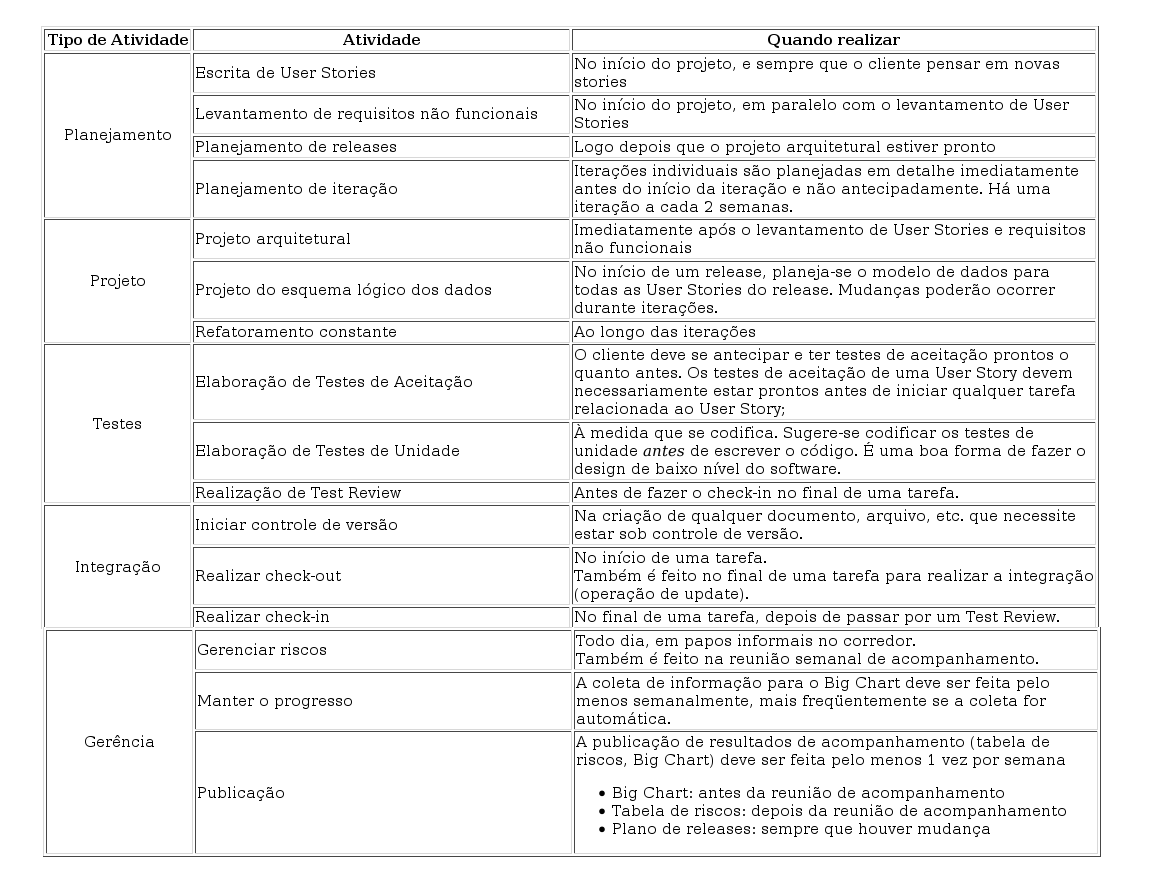
\includegraphics[height = 14cm]{tab1.png}
%  \caption{\it Tabela que descreve quando as atividades de XP1 devem ser realizadas.} \label{tab:tab1}
% \end{figure}

\begin{figure}[!h]
 \hfill
 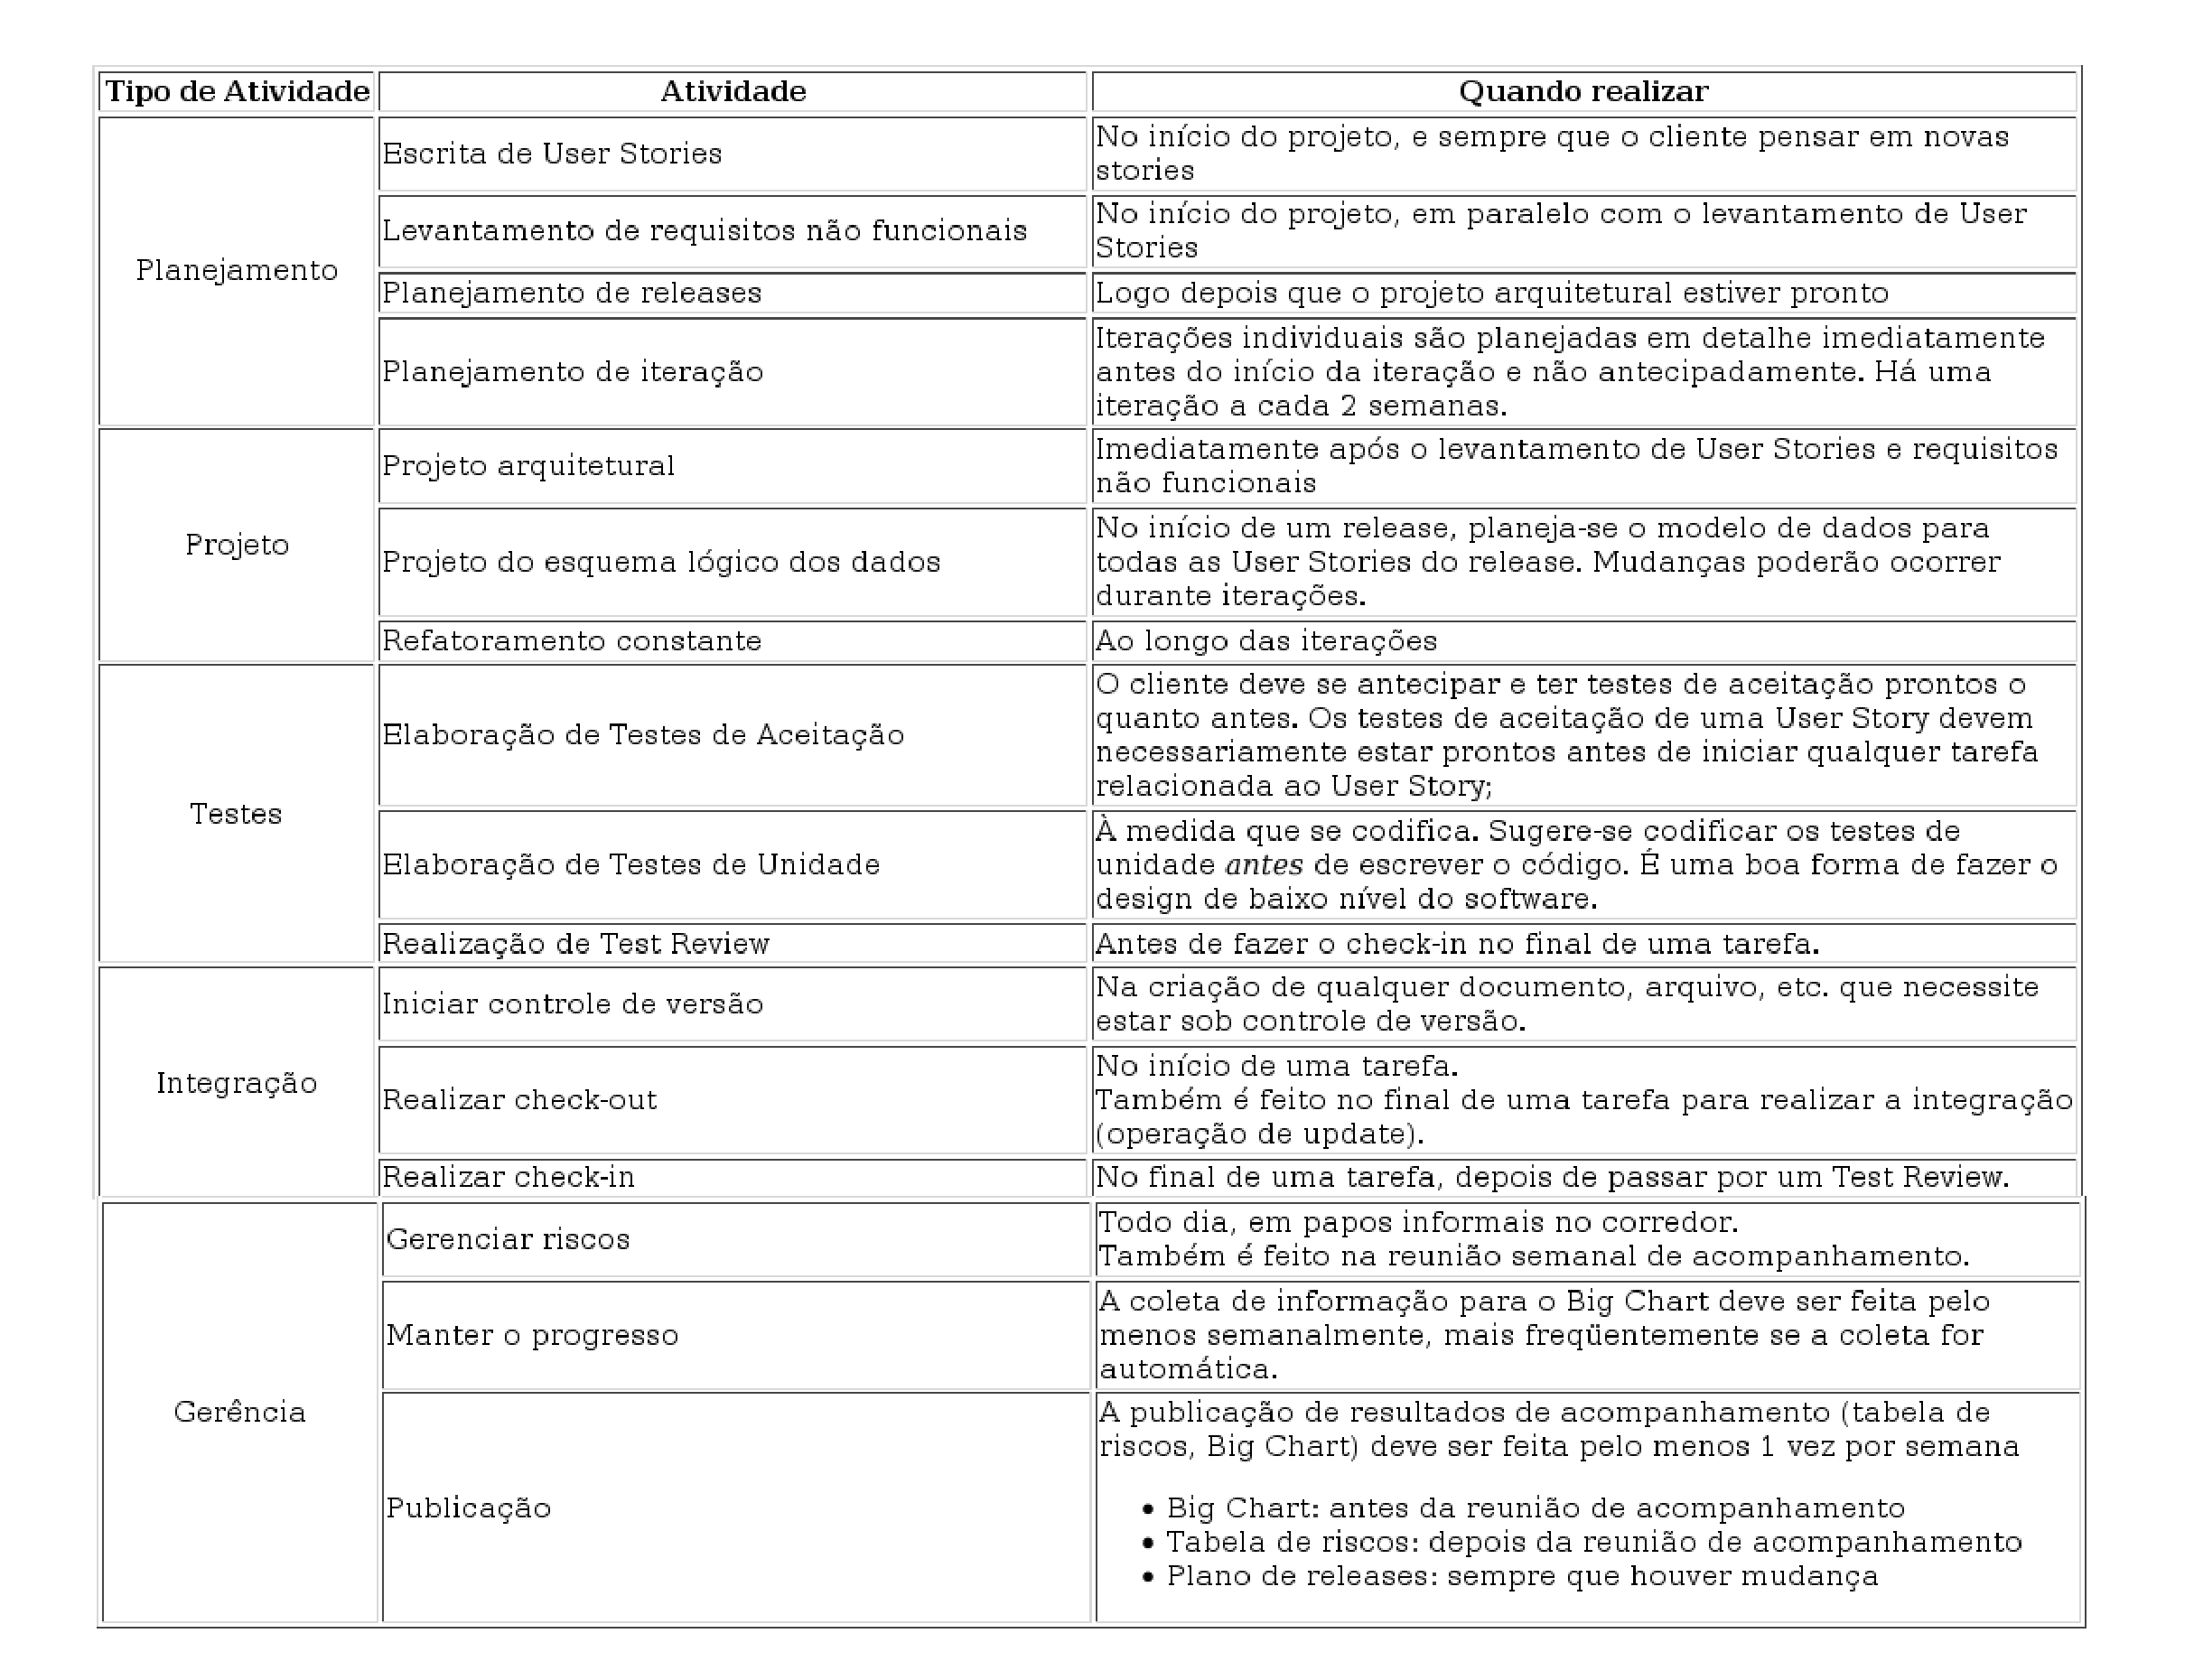
\includegraphics[height = 14cm]{tab1.eps}
 \caption{\it Tabela que descreve quando as atividades de XP1 devem ser realizadas.} \label{tab:tab1}
\end{figure}

%\begin{table}[h]
% \caption{Tabela que descreve quando as atividades de XP1 devem ser realizadas}
% \centering
% \begin{tabular}{c|l|l}
%  \hline \hline
%  Tipo de Atividade & Atividade & Quando Realizar\\
%  \\[0.5ex]
%  \hline
%  Planejamento & Escrita de User Stories; \cline{1-1}
%  Levantamento de requisitos não funcionais; 
  %Planejamento de releases; Planejamento de iteração 
%  & No início do projeto, e sempre que o cliente pensar em novas stories; \\
  %No início do projeto, em paralelo com o levantamento de User Stories;
  %Logo depois que o projeto arquitetural estiver pronto; 
  %Iterações individuais são planejadas em detalhe imediatamente antes do início da iteração e não antecipadamente;
  %Há uma iteração a cada 2 semanas.\\
%  z & 2
% \end{tabular}
%\end{table}

Instanciando os papéis identificados anteriomente (cliente, desenvolvedor e gerente) no contexto do projeto obtém-se a seguinte classificação: i) o professor Dr. Hyggo O. de Almeida assumiu o papel de cliente; ii) quanto ao papel de gerente, cada um dos integrantes da equipe assumiu a chefia do grupo por um determinado tempo durante o desenvolvimento (aproximadamente um mês cada); e iii) por tratar-se de um número reduzido de pessoal para execução do trabalho, durante o decorrer do projeto todos integrantes foram desenvolvedores/testadores.

Quanto à alocação de atividades (descritas na Tabela \ref{tab:tab1}), houve sempre a preocupação em dividi-las igualitariamente entre os membros da equipe. Para tal, reuniões de acompanhamento foram realizadas semanalmente. Nessas reuniões os membros da equipe procuravam alocar, segundo as habilidades de cada indivíduo, as atividades do modo mais adequado possível. Não havendo acordo, ficava a cargo do gerente da vez impor sua decisão final.

Adaptando as atividades elencadas pelo XP1 ao contexto do projeto percebe-se a seguinte configuração: 
\begin{itemize}
 \item  A atividade de planejamento consumiu bastante tempo ainda na primeira parte da disciplina de Projeto I, pois esta etapa envolveu uma ampla pesquisa na literatura especializada para verificação de quais requisitos, funcionais e não funcionais, deveriam estar presentes no produto final. Com os requisitos já identificados e com as \textit{User Stories} escritas, o próximo passo foi realizar o planejamento das iterações e \textit{releases}. É válido salientar que apesar de todo esse planejamento ter sido realizado durante as primeiras etapa do processo, a cada semana, durante as reuniões de acompanhamento, uma revisão sobre esses artefatos era realizada para garantir que o que se havia planejado realmente estava de acordo com a realidade do problema e da equipe. Portanto, alterações pontuais nos artefatos de planejamento foram realizadas durante todo o processo de desenvolvimento.
 \item A atividade de projeto foi iniciada imediatamente após a conclusão da etapa de planejamento. De posse das \textit{User Stories} e dos requisitos do sistema a equipe em conjunto montou o projeto arquitetural do sistema. O projeto arquitetural decidido foi simplificado, baseado pricipalmente nas ideias de MVC, porém atendeu as necessidades ali presentes. Quanto ao esquema lógico, por tratar-se de um projeto que não envolve grandes manipulações de dados, a equipe decidiu por não adotar um banco de dados, e apenas trabalhar com arquivos XML, quando necessário.
 \item Dada a importância que a atividade de testes tem para um bom produto final, a equipe buscou construir suites de teste de qualidade que pudessem localizar rapidamente possíveis deficiências do código. Para tal, logo que as \textit{User Stories} foram escritas os testes de aceitação das mesmas já começaram a ser desenvolvidos em sequência. E, seguindo o que indica a metodologia de testes TDD \cite{TDD}, os testes de unidade foram sempre desenvolvidos antes que a codificação fosse realizada. É importante destacar que como o projeto foi proposto para um cliente que não era da área financeira, os testes de aceitação foram escritos pelos desenvolvedores a partir de materiais de exercícios financeiros encontrados na Internet, incluindo os manuais da HP-12C \cite{man1} \cite{man2} \cite{man3} \cite{man4} e o material de matemática financeira do professor Adail Marcos Lima Da Silva \cite{adail}, e comparando-se os resultados com os resultados da HP-12C real. Outro ponto importante é que existiu sempre a preocupação de que pessoas diferentes escrevessem e revisassem os testes, procurando, assim, garantir uma maior credibilidade aos testes. 

 \item A atividade de integração foi uma preocupação constante da equipe desde a fase de planejamento. Para que não ocorressem divergências ou inconsistências de conteúdo, surgiu a preocupação de criar um controle de versões tanto para a biblioteca financeira quanto para a calculadora \textit{Pyfinancial}, para tal fez-se uso das já muito conhecidas ferramentas de controle de versões SVN \cite{SVN} e Garage \cite{garage}, respectivamente. Com isso, manteve-se um controle sistematizado do código, bem como dos artefatos de planejamento.

 \item Quanto à realização de \textit{Reviews}, sempre foi alocado um tempo após a escrita dos testes e do código funcional para a revisão da qualidade dos testes escritos (verificando novamente os resultados com a calculadora, observando coerência e cobertura dos mesmos, etc.), bem como para realizar algum refatoramento que se mostrasse necessário de maneira imediata. Embora tenha-se procurado organizar o design de maneira flexível, percebeu-se no decorrer do projeto que alguns pontos poderiam sofrer um refatoramento maior. Essa necessidade possivelmente está relacionada com o fato de não ter sido alocado desde o início um tempo maior para \textit{Code} e \textit{Design Review}.

 \item Por fim, como já dito anteriormente, a atividade de gerência foi revesada entre os membros da equipe. Cada um atuou como gerente por um determinado período de tempo durante a realização do projeto. Ao gerente coube entender as mudanças discutidas durante as reuniões de acompanhamento e refleti-las tanto nos artefatos de planejamento (\textit{User Stories}, requisitos, projeto arquitetural etc), quanto nos artefatos de gerência (\textit{Big-Chart}, a tabela de riscos  e o plano de \textit{realises} etc). Essa atividade foi realizada sempre em paralelo com o desenvolvimento da aplicação, aproximadamente uma vez a cada semana.
 
\end{itemize}

Para garantir que as atividades fossem realizadas da forma mais adequada possível uma infra-estrutura foi montada a fim de melhorar a organização e consequentemente a qualidade do código produzido. Dentre os elementos presentes nessa infra-estrutura podemos destacar:

\begin{itemize}
 \item \textbf{Eclipse} \cite{eclipse}. IDE de desenvolvimento.
 \item \textbf{PyDev} \cite{pydev}. \textit{Plug-in} para desenvolvimento em Python.
 \item \textbf{PyUnit} \cite{pyunit}. \textit{Framework} para desenvolvimento de testes de unidade.
 \item \textbf{PyEasyAccept} \cite{pyeasyaccept}. \textit{Framework} para desenvolvimento de testes de aceitação.
 \item \textbf{SVN e Garage SVN} \cite{SVN}\cite{garage}. Ferramentas para controle de versões
\end{itemize}


\chapter{Análise de Requisitos}
asasa


\chapter{Arquitetura}

% \begin{figure}[!h]
%  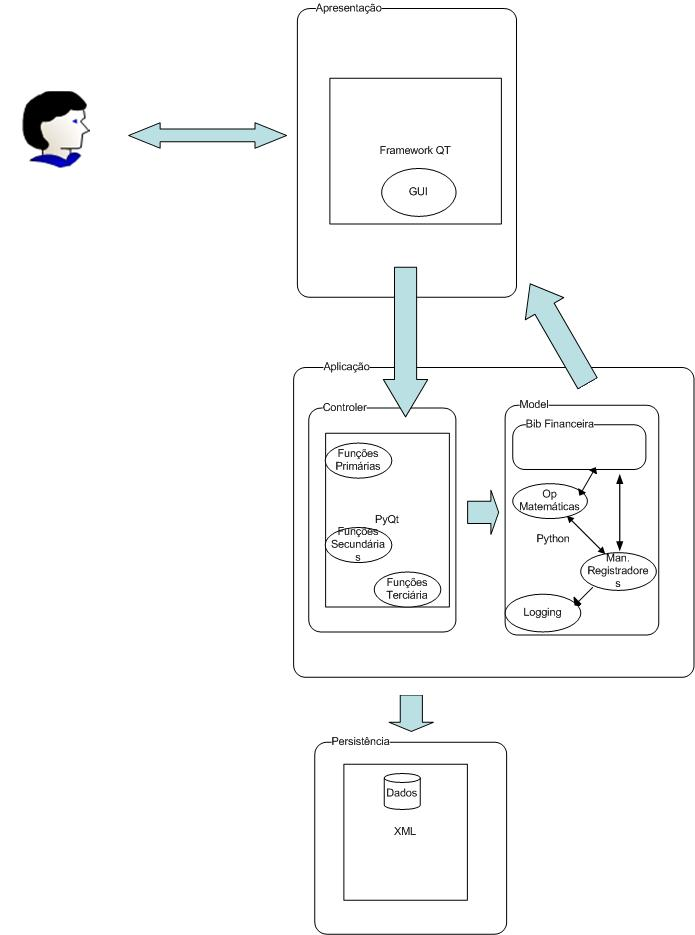
\includegraphics[scale=0.5]{arquitetura.jpg}
%  \caption{\it Projeto arquitetural da aplicação.} \label{fig:arquit}
% \end{figure}

\section{Descrição da Arquitetura}

O sistema proposto foi idealizado para funcionar localmente no dispositivo N800 da Nokia, funcionando no modo monousuário. O sistema pode ser dividido, em três camadas lógicas que serão conectadas através do padrão MVC \cite{mvc}, conforme pode ser visto na Figura \ref{fig:arquit}:
\begin{itemize}
 \item \textbf{Apresentação}: camada que será responsável por lidar com todo aspecto de interface para interação com o usuário.
 \item \textbf{Aplicação}: camada que será responsável por conter toda a lógica do negócio de nossa aplicação, mantendo, assim total desacoplamento com as demais camadas.
 \item \textbf{Persistência}: camada que será responsável por lidar com toda a persistência de dados de mode que eles possam ser usados posteriormente íntegros.
\end{itemize}

Vale lembrar que toda a comunicação entre essas camadas, bem como entre os diversos módulos internos as mesmas, é realizada através de um conjunto de interfaces bem definidas, buscando assim, garantir flexibilidade e baixo acoplamento, bem como um eventual reuso e/ou substituição da biblioteca financeira em questão. A separação estre os módulos se deu da forma mais simplificada possível para que não existisse maior sobrecarga que pudesse influenciar drasticamente o tempo de resposta desejados para as iterações com o usuário da aplicação, este foi um dos requisitos não-funcionais especificados na fase de análise.
Outro ponto importante a se destacar é o uso do paradigma OO, bem como do uso de scripts, dada a escolha da linguagem Python para o desenvolvimento da Camada de Aplicação.

\begin{figure}[!h]
 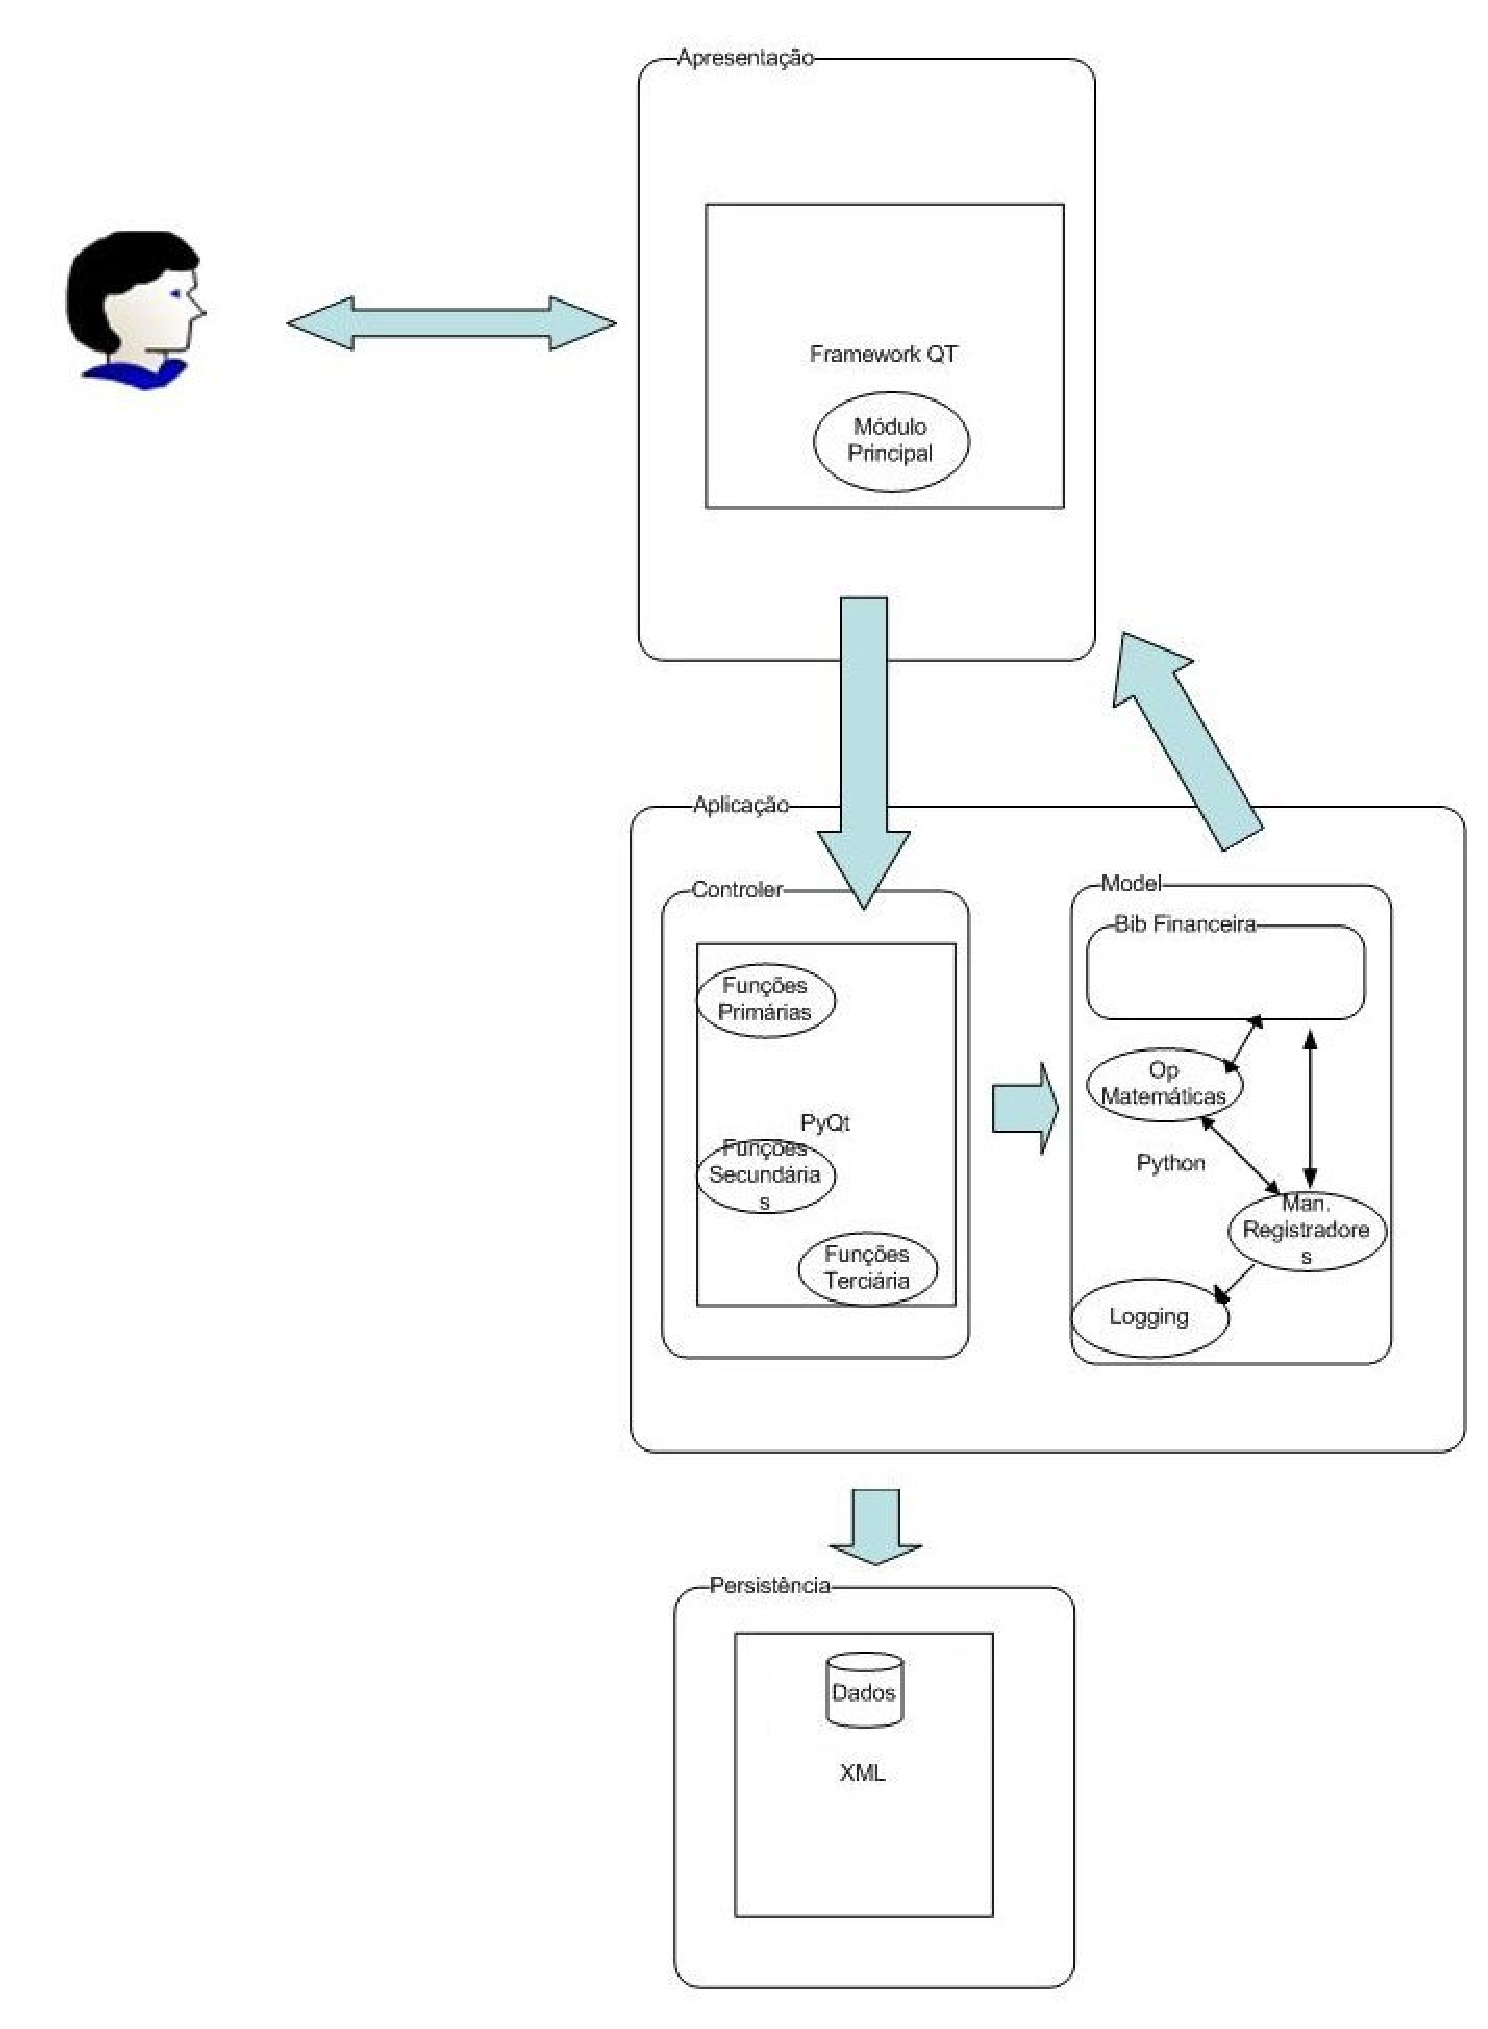
\includegraphics[scale=0.5]{arquitetura.eps}
 \caption{\it Projeto arquitetural da aplicação.} \label{fig:arquit}
\end{figure}

\subsection{Camada de Apresentação}
O sistema será acessado localmente por um único usuário via uma interface similar a da calculadora financeira que estamos usando como base, tendo a adição de menus de auxílio para uso do sistema e uma opção de finalização da aplicação. É importante destacar ainda que toda entrada realizada pelo usuário se dará através da interface touch-screen disponibilizada pelo dispositivo selecionado.
Para o desenvolvimento dessa camada faremos uso do Framework QT, com auxílio da ferramenta de design gráfico QT Designer. É de suma importância aqui o desenvolvimento de packages no que diz respeito aos componentes visuais da calculadora, por exemplo, os botões da mesma.

\subsection{Camada de Aplicação}
Como dito anteriormente, essa camada é responsável por toda a lógica de negócio de nosso sistema e foi desenvolvida em Python devido a suas vantagens na manipulação de números.
Dentre os principais componentes desta camada podemos dar destaque à biblioteca financeira (também desenvolvida por esta equipe com o foco de ser um módulo importável que contenha essencialmente funcionalidades financeiras), ao módulo de operações matemáticas, ao módulo de gerenciamento dos registradores existentes (responsável por fornecer os dados a serem persistidos) e ao módulo de comunicação com a interface da calculadora.
 Dentro dessa camada podemos destacar que as interações ocorrem em duas etapas:
\begin{enumerate}
 \item Numa primeira etapa teremos a comunicação dessa camada com a camada de apresentação do sistema através dos controladores, fazendo estes uso dos bindings em PyQt e sendo subdivididos de acordo com as funcionalidade providas por cada tecla.
 \item Numa segunda etapa teremos:	
 \begin{itemize}
  \item \begin{itemize}
         \item A comunicação dos módulos controladores com o restante da lógica da aplicação, fazendo uso das funcionalidades da biblioteca financeira, do módulo matemático e manipulando os seus registradores.
	 \item A interação entre os registradores e a biblioteca, onde os primeiros podem fornecer entradas para a última, a interação entre os registradores e o módulo matemático e a interação entre o módulo matemático e a biblioteca.
        \end{itemize}
 \end{itemize}
\end{enumerate}

\subsection{Camada de Persistência}
A persistência dos dados relativos aos registradores é realizada através do uso de arquivos. Os dados que forem armazenados nos arquivos deverão ser recarregados sempre que houver a inicialização da aplicação, demandando, assim, pouca interação com o disco.
Outro aspecto relevante a ser considerada aqui é a segurança do sistema.  Devido à natureza do sistema focamos nos aspectos de integridade dos dados manipulados, fazendo com que os arquivos utilizados fossem armazenados de forma oculta ao usuário, evitando, assim, alterações dos mesmos por parte deste.

\subsection{\textit{Packing}}
Foi tomada a decisão de distribuir a aplicação através de um arquivo de instalação de extensão .deb, simplificanco assim a maneira de intalação do software. Tal arquivo poderá ser obtido por download de certo servidor web que será escolhido pela equipe em conjunto com o cliente.

\subsection{Pontos Adicionais}
Com relação à integração com outras aplicações, é do interesse da equipe que a biblioteca financeira desenvolvida possa vir a ser usada por outros desenvolvedores como um dos vários módulos que auxiliem sua aplicação específica.
Por fim, todo nosso desenvolvimento foi guiado pelo padrão de operações que é usado pela HP12-C que é a Notação Polonesa Reversa, ou Inversa segundo alguns autores \cite{NPR}



\chapter{Verificacao e Validacao}
dsdsd


\chapter{Métricas}

Dentre as várias formas que um gerente de projeto tem a sua disposição para acompanhar o andamento de um projeto podemos destacar o uso de um \textit{Big Chart}. O mesmo pode ser visto como a análise quantitativa do andamento do projeto. As métricas a serem apresentadas são escolhidas pelo gerente e buscam refletir que pontos deseja-se acompanhar, por exemplo, se número de classes, número de linhas de código, testes de unidade que estão rodando perfeitamente, etc. As métricas escolhidas pela equipe em questão foram:

\begin{itemize}
 \item Número de Módulos python
 \item Número de scripts
 \item Número de Scritps de Testes de Aceitação Implementados e Executando Corretamente
 \item Número de Módulos de Testes de Unidade Implementados e Executando Corretamente
 \item Número de User Stories Finalizadas
 \item Total de Linhas de Código
 \item Total de Linhas de Teste
\end{itemize}


Vale ressaltar que o \textit{Big Chart} faz parte da documentação especificada em alguns processos vistos na academia como o \textit{YP} \cite{yp} e o \textit{XP1} \cite{xp1}. Como o processo de desenvolvimento escolhido durante as disciplinas de Projeto I e Projeto II foi baseado no \textit{XP1}, o \textit{Big Chart} foi utilizado para acompanhamento em alto nível do projeto por parte do cliente, bem como dos integrantes da equipe de desenvolvimento

Uma vez que as iterações foram definidas com duração de 15 dias e uma release contemplou, em média, duas iterações, optou-se em Projeto I por gerar as métricas a cada release. Entretanto, como no final da disciplina surgiu um grave problema de convergência no resultado das fórmulas que estavam sendo usadas até então, optou-se por alterar o intervalo de atualização do mesmo, passando agora a atualizá-lo a cada 15 dias. Com isso buscou-se um maior controle sobre o status do projeto.

\begin{figure}[!h]
\subfigure[Métricas Gerais\label{fig:geral}]
{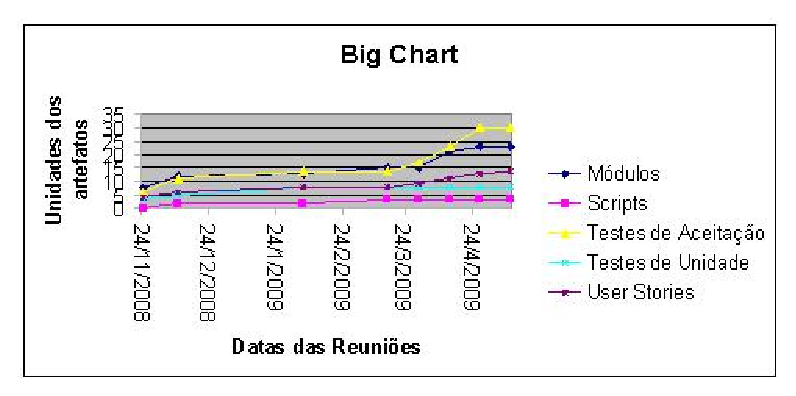
\includegraphics[scale = .8]{bc.eps}}
\subfigure[Linhas de código\label{fig:loc}]
{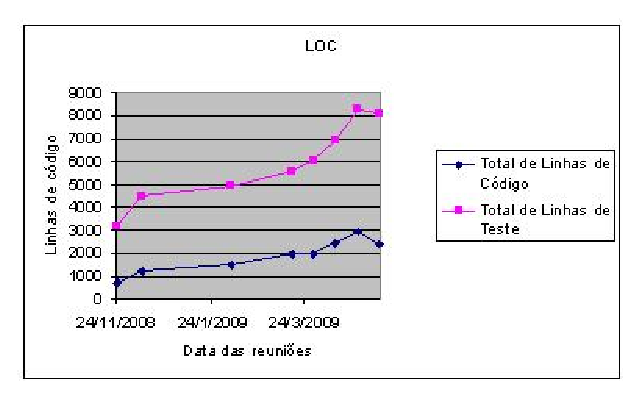
\includegraphics[scale = .8]{bc2.eps}}
%  \includegraphics[scale=0.5]{bigchart.eps}
 \caption{\it Big Chart.} \label{fig:bigchart}
\end{figure}

Conforme pode-se observar nas Figuras \ref{fig:geral} e \ref{fig:loc}, o desenvolvimento apresentou-se crescente até os meses de Fevereiro e Março quando o problema acima citado foi encontrado. Nesse instante foi realizado uma pesquisa por novas fórmulas, com teste das mesmas, o que levou a uma estabilidade tanto no total de linhas de código, como no número de scripts, módulos, testes de aceitação, testes de unidade e user stories. Nesse mesmo intervalo o aumento no total de linhas de teste se deve à especificação de uma maior quantidade de testes de modo a garantir uma maior convergência com os resultados da HP-12C.

Durante o mês de Março, uma vez encontrado um conjunto de fórmulas que propiciou uma convergência adequada, iniciou-se o desenvolvimento das demais user stories em questão e por isso explica-se o crescimento das métricas avaliada. As últimas avaliações realizadas em maior apresentam valores constantes na Figura \ref{fig:geral} dado que esse foi um período de refatoramento de código e testes, bem como de melhorias em aspectos da interface. É interessante ressaltar que as alterações aqui produzidas levaram a uma certa queda no total de linhas de código e testes, Figura \ref{fig:loc}, dado que foi observado certa redundância em trechos de código e teste, bem como o fato de que foram realizadas simplificações na interface, o que leva a um menor número de linhas de código.

Outro ponto que merece explicação é o porquê da quantidade de linhas de teste ser tão superior à quantidade de linhas de código. Mediante o uso do framework QT e da linguagem Python, bem como da busca de uso de boas técnicas de programação e design, o código da aplicação tornou-se bastante enxuto e reduzido. Quanto aos testes, uma vez que buscou-se uma grande similaridade com os resultados da HP-12C, foi elaborada uma alta carga de testes, buscando contemplar a maior variedade de cenários possível no tempo de desenvolvimento proposto.





\chapter{Conclusões e Trabalhos Futuros}

Um dos méritos desse projeto foi trabalhar com conhecimento multidisciplinar, envolvendo 
conhecimentos adquiridos em disciplinas de computação, como Engenharia de Software, Métodos de
Software Numérico e Sistemas de Informação um e dois, assim como em disciplinas extras, como
Princípios de Administração Financeira. Dessa forma, os integrantes da equipe tiveram a
oportunidade de exercitar o conhecimento adquiridos em sala de aula.

A opção por desenvolver uma aplicação para dispositivos móveis também contribuiu para o amadurecimento
da equipe no tocante a perceber as particularidades e as dificuladades de se trabalhar no desenvolvimento desse tipo
de sistema. Além disso, essa experiência possibilitou o contato com diversas novas tecnologias,
aumentando o conhecimento da equipe e inserindo diferenciais nos currículos profissionais.

Uma das dificuldades enfrentadas pelo grupo foi a falta de apoio na área financeira. O cliente
cumpriu muito bem o seu papel, porém este tinha maior embasamento na área de dispositivos móveis.
Houveram diversas tentativas, por parte do grupo e do cliente, em obter um apoio na área financeira,
porém com pouco sucesso.

Como trabalhos futuros, planejamos a adição de novas fórmulas financeiras, bem como o refatoramento
das fórmulas existentes para introduzir métodos melhores para calcular os resultados. Planeja-se
também trabalhar em melhorias na interface com o usuário, visto que isso não foi possível no
decorrer das disciplinas pois a biblioteca gráfica utilizada ainda estava em processo de migração
para a plataforma Nokia Maemo.

Enfim, toda a experiência vivida em Projeto I e II possibilitou o crescimento dos alunos como
desenvolvedores, analistas e gerentes de projeto. Aguçando as habilidades de resolução
de problemas e permitindo o contato com novos conceitos e paradigmas.


\appendix
\chapter{Glossário} \label{glossario}

\textbf{A}

\begin{itemize}
\item Amortização:
    A palavra amortização pode ser entendida como a diminuição da dívida, de uma única vez ou aos poucos, em mais vezes. 
\end{itemize}

\textbf{C}
\begin{itemize}
\item Capitalização: 

    Periodicidade do vencimento do juro ou número de vezes em que o juro é processado (calculado) num ano: anual, semestral, trimestral, mensal, etc. 

\item Capitalização Linear:
    A capitalização linear – ou método de formação dos juros simples – considera a incidência periódica de uma dada taxa de juros sobre uma base de cálculo fixa. 

\item Capitalização exponencial:
    A capitalização exponencial ou – método de formação dos juros compostos – considera a incidência periódica de uma dada taxa de juros sobre uma base de cálculo variável. 

\item Capital inicial:
    Capital existente na data-pólo inicial. 

\item Capital final:
    Capital existente na data-pólo final. 

\end{itemize}

\textbf{D}
\begin{itemize}
 \item Data-pólo inicial:
    Data de início do investimento. 

\item Data-pólo final:
    Data de resgate do investimento. 

\item Datas-focais intermediárias:
    Datas localizadas entre a data-pólo inicial e a data-pólo final, onde existem movimentações financeiras. 

\item Diagrama de tempo:
    Diagrama que apresenta o fluxo de caixa juntamente com os instantes de tempo das movimentações. Por convenção, recebimentos, entradas ou fluxos positivos são representados por setas apontando para cima ao passo que saídas ou pagamentos ou fluxos negativos são representados por setas apontando para baixo. 
\end{itemize}

\textbf{F}
\begin{itemize}
 \item Fluxo de Caixa:
    Montante de caixa recebido e gasto por uma entidade durante um período de tempo definido, algumas vezes ligado a um projeto específico. 
\end{itemize}

\textbf{J}
\begin{itemize}
 \item Juros de uma prestação em um sistema de amortização:
    Quantia paga além do valor amortizado em cada parcela. É calculada em função da taxa de juros e do saldo devedor do instante anterior. 

\item Juros Simples:
    No sistema de juros simples, os juros são calculados sobre o principal da dívida (valor inicial emprestado ou aplicado) 

\item Juros Compostos:
    No sistema de juros compostos, os juros de cada período somam-se à dívida, incidindo juros sobre ele no período seguinte 
\end{itemize}

\textbf{P}
\begin{itemize}
 \item Pagamento Antecipado:
Pagamento de uma prestação que é realizado no início de um dado período.

\item Pagamento Postecipado:
Pagamento de uma prestação que é realizado no término de um dado período.

\item Prestação:
    Instrumento de recuperação ou de devolução de um capital acrescido dos juros contratados no período de negociação da transação. 
\end{itemize}

\textbf{S}
\begin{itemize}
 \item Saldo Devedor:
    Montante que ainda necessita ser abatido em um dado instante de tempo considerando um certo sistema de amortização. 

\item Série Simples:
    Quando um fluxo de caixa apresenta apenas datas-pólo, ou seja, temos apenas dois fluxos. 

\item Série Complexa:
    Quando um fluxo apresenta ao menos uma data-focal intermediária além das datas-pólo, ou seja, tem-se no mínimo três fluxos. 

\item Série Uniforme de Prestações Uniformes:
    Conjunto de pagamentos ou recebimentos nominais iguais, dispostos em períodos constantes ao longo de uma série complexa de fluxo de caixa. Pode ser de três tipos: postecipada, antecipada ou diferida. 

\item Série Uniforme de Prestações Uniformes Antecipada:
    São pagamentos ou recebimentos distribuídos por todos os períodos de uma série complexa de fluxo de caixa, inclusive na data-pólo inicial ou data-focal zero. 

\item Série Uniforme de Prestações Uniformes Diferida:
    São pagamentos ou recebimentos distribuídos em uma série complexa de fluxo de caixa por períodos situados após um determinado prazo de carência. 

\item Série Uniforme de Prestações Uniformes Postecipada:
    São pagamentos ou recebimentos distribuídos por todos os períodos de uma série complexa de fluxo de Caixa, menos na data-pólo inicial ou data-focal zero. 

\item Sistema de Amortização:
    É a forma pela qual são calculadas as prestações que você vai pagar no decorrer do financiamento. Nos empréstimos de longo prazo, esses pagamentos são, normalmente, efetuados por parcelas (prestações), compostas de cotas de amortização e de juros. 

\item Sistema de Amortização Constante:
    É um método onde as amortizações do capital apresentam comportamento uniforme ou constante durante o período de vigência de uma operação financeira. Os juros apresentam valores heterogêneos e decrescentes ao longo do tempo, o que resulta em prestações heterogêneas e decrescentes ao longo do tempo. 

\item Sistema de Amortização Mista:
    Criado em 1979 pelo BNH. Representa um plano de amortização misto, a partir da combinação entre os sistemas Francês e Constante, onde juros, amortização e prestação, derivam de médias aritméticas envolvendo os valores calculados no PRICE e no SAC. Os juros apresentam valores heterogêneos e decrescentes ao longo do tempo. Com os juros heterogêneos e amortizações homogêneas temos uma configuração de prestações heterogêneas e decrescentes. 

\item Sistema Francês:
    Criado no século XVIII pelo matemático, filósofo e teólogo inglês Richard Price (por isso o nome Sistema Price), é um método de amortização com prestações iguais e vencidas, onde juros e amortizações portam-se de maneiras decrescente e crescente. 
\end{itemize}

\textbf{T}
\begin{itemize}
\item Taxa de Juros:
    É o percentual que remunera o capital. Uma taxa de juros incide sobre um capital disposto em um fluxo de caixa sempre quando da ocorrência de uma variação temporal, conhecida como freqüência intervalar necessária à formação dos juros 
\end{itemize}

\textbf{V}
\begin{itemize}
 \item Valor Atual ou Valor Presente:
    Representa um fluxo qualquer situado na data-pólo inicial. 

\item Valor Nominal
    Representa um fluxo qualquer situado entre a data-focal intermediária 1 e a data-pólo final. 

\item Valor Futuro Antecipado:
    Representa o somatório de todas as prestações capitalizadas à data-pólo final, com uma mesma taxa de juros; o PMT contido na data-pólo final não sofre nenhuma alteração 

\item Valor Futuro Postecipado:
    Representa o somatório de todas as prestações capitalizadas à data-pólo final, 
com uma mesma taxa de juros.

\item Valor Presente Antecipado:
    Representa o somatório de todas as prestações descontadas à data-pólo inicial, com uma mesma taxa de juros; o PMT data-pólo inicial não sofre nenhuma alteração 

\item Valor Presente Postecipado:
    Representa o somatório de todas as prestações descontadas à data-pólo inicial, com uma mesma taxa de juros. 
\end{itemize}
\chapter{Fórmulas}

Aqui serão apresentadas as fórmulas usadas, bem as fontes a partir das quais as mesmas foram obtidas: \\

\begin{enumerate}
 \item pv - BEG \cite{arachnoid}:

\begin{eqnarray*}
pv &=& (i+1)^{-n} * ( -fv*i - (i+1) * ( (i+1)^{n} -1)*pmt  ) / i\\
\end{eqnarray*}

% Fonte: http://www.arachnoid.com/lutusp/finance.html

\item pv - END \cite{arachnoid}:

\begin{eqnarray*}
	pv &=& (i+1)^{-n} * ( -pmt*(i+1)^{n} - fv*i + pmt) / i \\
\end{eqnarray*}

%  Fonte: http://www.arachnoid.com/lutusp/finance.html

\item pv com i = 0 \cite{matFinanceira}: 

\begin{eqnarray*}
  pv &=& fv + n * pmt  \\
\end{eqnarray*} 

% Fonte: Material de Camilo e \cite{matFinanceira}

\item fv - BEG \cite{arachnoid}:
\begin{eqnarray*}
 fv &=& ( (i+1)*pmt - (i+1)^{n}*(i*pmt + pmt + i*pv) ) / i \\
\end{eqnarray*}

%  Fonte: http://www.arachnoid.com/lutusp/finance.html

\item fv - END \cite{arachnoid}: 
\begin{eqnarray*}
fv &=& ( pmt - (i+1)^{n} * (pmt + i*pv) ) / i \\
\end{eqnarray*}

%  Fonte: http://www.arachnoid.com/lutusp/finance.html 

\item fv com i = 0 \cite{arachnoid2}:
\begin{eqnarray*}
 fv &=& - (pv + n*pmt) \\
\end{eqnarray*}
 
%  Fonte: Material de Camilo e \cite{matFinanceira}

\item  n - BEG \cite{arachnoid}:
\begin{eqnarray*}
 n &=& log( (-fv*i + pmt*i + pmt) / (i*pmt + pmt + i*pv) ) / log(i+1) \\
\end{eqnarray*} 

%   Fonte: http://www.arachnoid.com/lutusp/finance.html 

\item  n - END \cite{arachnoid}: 
\begin{eqnarray*}
 n &=& log( (pmt - fv*i) / (pmt + i*pv) ) / log(i+1) \\
\end{eqnarray*} 
  
%  Fonte: http://www.arachnoid.com/lutusp/finance.html

\item  n com i = 0 \cite{arachnoid2}: 

\begin{itemize}
 \item Se pólos com sinal igual:
	\begin{eqnarray*}
 		 n &=& |(pv - fv)| / |pmt| \\ 		
	\end{eqnarray*}
  \item c.c:
	\begin{eqnarray*}
 		n &=& (|pv| - |fv|) / |pmt|   ^{1} \\	 
	\end{eqnarray*}
\end{itemize}
 
%  Fonte: Material de Camilo e \cite{matFinanceira} \\

\item  pmt - BEG \cite{arachnoid}: 
\begin{eqnarray*}
	pmt &=& - i*( pv* ( i+1 )^{n} + fv ) / ( (i+1)*( (i+1)^{n} - 1 ) ) \\
\end{eqnarray*} 
 
%  Fonte: http://www.arachnoid.com/lutusp/finance.html \\ 

\item  pmt - END \cite{arachnoid}:
\begin{eqnarray*}
	pmt &=& - i*( pv*(i+1)^{n} + fv ) / ((i+1)^{n} - 1) \\	
\end{eqnarray*}  
 
%  Fonte: http://www.arachnoid.com/lutusp/finance.html \\

\item  pmt com i = 0 \cite{arachnoid2}:  

\begin{itemize}
 \item Se pólos com sinal igual:
	\begin{eqnarray*}
 		 pmt &=& |(pv - fv)| / |n| \\	
	\end{eqnarray*}
  \item c.c:
	\begin{eqnarray*}
 		pmt &=& (|pv| - |fv|) / |n|  ^{1} \\	 
	\end{eqnarray*}
\end{itemize}

%  Fonte: Material de Camilo e \cite{matFinanceira}  

\item  i: Usa-se a função do fv com estimativas de i $ ^{2} $  \cite{arachnoid2}

%  Fonte: http://vps.arachnoid.com/finance/

\item  npv \cite{man1}:
\begin{eqnarray*}
 	NPV &=& CF_{0} + CF_{1} / (1+i)^{1} + CF_{2} / (1+i)^{2} + ... + CF_{n} / (1+i)^{n} \\
\end{eqnarray*}
 
%  Fonte: Manual da HP c00363319

\item  irr \cite {matFinanceira2}: Utilizado o método da secante para achar um valor de taxa na fórmula do $NPV$ em que $ NPV = 0. $ 

%  Fonte: Matemática Financeira de Samuel Hazzan e José Nicolau Pompeo

\item SAF: pmt \cite{adail}
\begin{eqnarray*}
 	pmt &=& pv * (1+i)^{n} * i / ((1+i)^{n}-1) \\
\end{eqnarray*}
 
%  Fonte: Material Adail

\item  SAF: amort \cite{adail}
\begin{eqnarray*}
 	A_{t} &=& (pmt - (pv*i)) * (i+1)^{t-1} \\	
\end{eqnarray*}
 
%  Fonte: Material Adail

\item  SAC: juros \cite{adail}
\begin{eqnarray*}
 	J_{t} &=& pv*i - (A_{t}*i*t-1)	
\end{eqnarray*}
 
%  Fonte: Material Adail 

\item  SAC: pmt \cite{adail}
\begin{eqnarray*}
 	pmt_{t} &=& A_{t} + J_{t}	\\
\end{eqnarray*}
 
%  Fonte: Material Adail

\item  SAC: amort \cite{adail}

\begin{eqnarray*}
 	A_{t} &=& pv / n \\	
\end{eqnarray*}
 
%  Fonte: Material Adail

\item  Conversão do n \cite{man2}:
\begin{eqnarray*}
 	n_{mensal} &=& n_{anual} * 12 \\	
\end{eqnarray*}
 
%  Fonte: Manual da HP Platinum em Português

\item  Conversão do i (juros simples) \cite{camilo}:
\begin{eqnarray*}
 	i_{mensal} &=& i_{anual} / 12 \\	
\end{eqnarray*}
  
%  Fonte: Material de Camilo de taxas equivalentes

\item  Conversão do i (juros compostos) \cite{camilo}:
\begin{eqnarray*}
 	i_{mensal} &=& (1+i_{anual})^{1/12} - 1 \\	
\end{eqnarray*}
 
%  Fonte: Material de Camilo de taxas equivalentes

\item Percentagem de um dado valor \cite{man1}:
\begin{eqnarray*}
 	\% &=& Base(y) * Rate(x) / 100 \\	
\end{eqnarray*}

\item Variação Percentual \cite{man1}:
\begin{eqnarray*}
 	\Delta\% &=& 100*(NewAmount(x)-Base(y))/Base(y) \\	
\end{eqnarray*}

\item Percentagem do Total \cite{man1}:
\begin{eqnarray*}
 	\%T &=& 100*(Amount(x)/Total(y)) \\	
\end{eqnarray*}

\end{enumerate}

Observações: 

$ ^{1} $ : Faz-se ainda um novo cálculo do pv com o valor resultante do n. Se o valor retornado for diferente, inverte-se o sinal do n.

$ ^{2} $ : O algoritmo base inicia com uma taxa de juros de 100\% e iterativamente, no máximo duas iterações mais externas trocando o sinal da taxa ou até achar a solução busca-se um novo valor de i. Internamente tenta-se acrescer uma estimativa atual de um valor gd, alterado de 0.5 ou -0.5 de acordo com certas condições, e verifica-se a proximidade do resultado dessa estimativa na função do fv em relação ao valor real do fv. Realizando-se três tentativas consecutivas de cálculo de fv que fiquem com um erro inferior a $ 1e-8 $ para-se o algoritmo, ou então tenta-se um número máximo de 400 iterações internas em estimativas do i.
\chapter{Novas Funcionalidades}

Dentre as várias características de um software bem projetado, pode-se ressaltar que uma das desejadas é permitir facilmente a inclusão de novas funcionalidades. Para isso elabora-se um bom design do mesmo, bem como uma boa documentação. Com esse intuito aqui será apresentado um pequeno guia que serve de auxílio para inclusão de novas funcionalidades, bem como para um melhor entendimento do sistema.

\section{Adicionando uma função}

\subsection{Considerações Iniciais}

Inicialmente serão destacados alguns esclarecimentos básicos a respeito da organização do código fonte:

\begin{enumerate}
 \item Em relação a interface gráfica, o módulo principal que organiza os dados de interface gráfica da calculadora, incluindo a disposição de botões, é o CalcGui. Além desse, existem módulos que lidam com a tabela de amortização (calcTableDialog), com a tabela de recall (recallViewDialog) e com a tabela de store (storeViewDialog). 

\item Existe um componente que representa um botão (calcButton). Para cada botão pode-se adicionar até 3 textos de funções: uma na parte superior, um na parte inferior e um na parte central.

\item O controller (calcController) captura todos os eventos de teclas pressionadas. A identificação das teclas se dá considerando o texto da parte central do botão 
(que representa a função principal de cada tecla). Em seguida o controller chama uma ação correspondente no model (calcModel).

\item O calcModel é a lógica de negócio do sistema. Esse módulo guarda o estado da calculadora (opções de arredondamento, se as teclas especiais f ou g estão pressionadas, etc) e conhece a pilha (calcStack), os demais registradores (calcRegs) e as funções da biblioteca financeira (pyFinancialLibrary).

\item O calcModel oferece publicamente funções que casam com as funções tidas como principais de cada botão (a funcão cujo texto fica no meio do botão). Dado que o calcModel conhece o estado da calculadora, em cada uma dessas chamadas verifica-se que função da biblioteca usar analisando, por exemplo, se o usuário selecionou os botões F ou G.

\item Na ligação do modelo, da interfaçe gráfica e do controlador foi utilizado o modelo MVC \cite {mvc}. Os módulos da interface gráfica atuam como \textit{Observers} da lógica de negócio e assim são ativados pela mesma quando necessários. O model tem vários listeners para eventos como: modificação do valor da tela, modificação da pilha, etc. A ativação de cada um desses listeners ocorre ao final de cada função do model, bem como a análise de outras ações necessárias como, por exemplo desativar a seleção de F ou G feita pelo usuário.
% ; avisar listeners sobre alterações na pilha, registradores financeiros, etc, 
% dependendo do que a função faça; alertar a interface sobre modificação na tela, no estado dos botões ou sobre 
% a necessidade de mostrar a tabela de amortização, de recall ou de store.

\item Os dados fornecidos de volta aos listeners estão sempre no tipo Decimal, que é o tipo trabalhado pela calculadora de modo a alcançar alta precisão. Cada módulo da GUI formata esses dados como queira, fazendo uso das funções de formatacão presentes no módulo calcFormatUtil.

\end{enumerate}

Um complemento do que foi exposto aqui pode ser analisado avaliando-se os diagramas de classes presentes no apêndice \ref{DiagramaClasses}.

\subsection{Exemplo de Adição de Função}

% Agora, como exemplo, irá se utilizar a implementação de uma nova forma de divisão em que ao invés de se dividir o 
% registrador Y pelo X, irá se dividir X por Y. Através desse exemplo, pretende-se abordar todo o passo-a-passo para se 
% implementar uma nova funcionalidade.
De modo a esclarecer melhor os pontos acima levantados, será simulada a implementação de uma nova funcionalidade na calculadora. Como exemplo, tem-se a adição de uma nova forma de divisão em que ao invés de se dividir o registrador Y pelo X, irá se dividir X por Y. 
Através desse exemplo, pretende-se abordar o passo-a-passo para se implementar uma nova funcionalidade no sistema em questão, considerando o caso simples de adição de uma função como principal em um dado botão.

Primeiramente é preciso escolher um botão do teclado da GUI que esteja livre para receber a nova função, ou ainda substituir uma função já alocada a algum botão. No método \begin{verbatim} __createKeyboardLayout \end{verbatim} do módulo calcGui é feita a adição de botões na tela. Nesse método deve-se escolher uma posição e adicionar o novo botão através do comando \begin{verbatim}self.__addGridButton(grid, "INV /", 1, 5)\end{verbatim}.

Em seguida, deve-se criar a ação a ser disparado no clique do botão. Para isso adiciona-se uma nova verificação do label central do botão pressionado no método \textbf{keyboardButtonClicked(self, text)} do controller. Um exemplo pode ser observado no trecho de código \ref{else}: 

\lstinputlisting[language=Python, label=else, caption={Teste no controller}]{else.py}
% \begin{verbatim}
% 	elif text == "INV /":
%  		self.__model.invDiv()
% \end{verbatim}

No model deve-se criar a função chamada no controller conforme visto acima. Na nova função do model implementa-se a funcionalidade considerando o estado dos botões 
F e G, os valores dos registradores, o estado da calculadora e as funções disponíveis na biblioteca de funções (pyFinancialLibrary). 

Com o resultado da divisão em mãos, altera-se o valor de algum(ns) dos registradores conforme necessário. Conforme dito acima, ao final de cada função deve-se, se necessário, desativar as teclas F e G, alterar a posição de entrada de decimais, e conforme o que for modificado (tela, pilha, registradores financeiros, etc) avisar os devidos listeners os novos valores que lhes são de interesse. 

Um ponto importante é também alterar o modo de entrada de dados da calculadora de acordo com a funcionalidade desejada. Existem basicamente três modos, explicitados na classe Mode: Mode.SaveMode (que na próxima entrada de dados devolve o valor 0.0 a tela e então inicia o processamento do que for entrado), Mode.OperationMode (devolve o valor zero a tela, mas antes dá um enter na pilha) e Mode.EntryMode (indicando que novos dígitos estão sendo entrados ao valor anterior da tela). 

Uma implementação de implementação da nova função de divisão no calcModel pode ser observado no trecho de código \ref{funcao}.

\lstinputlisting[language=Python, label=funcao, caption={Definição de Função no Model}]{funcao.py}


% \begin{verbatim}
% 
%     def invDiv(self):
%         if self.__isGPushed or self.__isFPushed:
%             self.__fireException("Function not yet implemented.")
%             self.__deactiveFandG()
%         else:
%             # "inv /"
%             try:
%                 result = self.__calcStack.getXReg() / self.__calcStack.getYReg()
%                 self.__calcStack.rollCounterClockWise()
%                 self.__calcStack[0] = result
%                 self.__calcStack[3] = self.__calcStack[2]
%         
%                 self.mode = Mode.OperationMode
%                 self.base = None
%                 self.dotActived = False
%         
%                 self.__fireStackRegisters(self.getAllStackRegisters())
%                 self.__fireScreenChangedEvent()
%                  
%             except Exception, e:
%                 self.__fireException(e.message)
% \end{verbatim}

\chapter{Tabela de Erros} \label{tabelaErros}

Como sabe-se sistemas apresentam restrições quanto as entradas fornecidas de modo a realizar determinadas atividades. Na HP-12C entradas inválidas produzem erros que são a\-presentados ao usuário através de um código no formato \textbf{ERROR d+}, onde d+ indica um ou mais dígitos. Esse formato dificulta o entendimento por parte do usuário do motivo que levou ao erro, ou seja, o usuário necessita ter em mãos o manual da calculadora que explicita o significado do código visualizado.

Nesse sentido, buscou-se fazer uso das facilidades que o dispositivo computacional em foco oferece de modo a melhorar a usabilidade do sistema. Para isso foi realizado um mapeamento dos códigos de erros encontrados nos cálculos financeiros na HP-12C para mensagens de texto que explicitem melhor o problema encontrado. 

Como a aplicação desenvolvida é composta de uma biblioteca financeira que é utilizada pela aplicação calculadora financeira, optou-se por realizar dois mapeamentos: um das mensagens que são geradas pelos cálculos financeiros da biblioteca e outro das mensagens que são geradas por estados inconsistentes na calculadora. Tais mapeamentos estão presentes nas tabelas \ref{tabErros1} e \ref{tabErros2}.

\begin{figure}[!h]
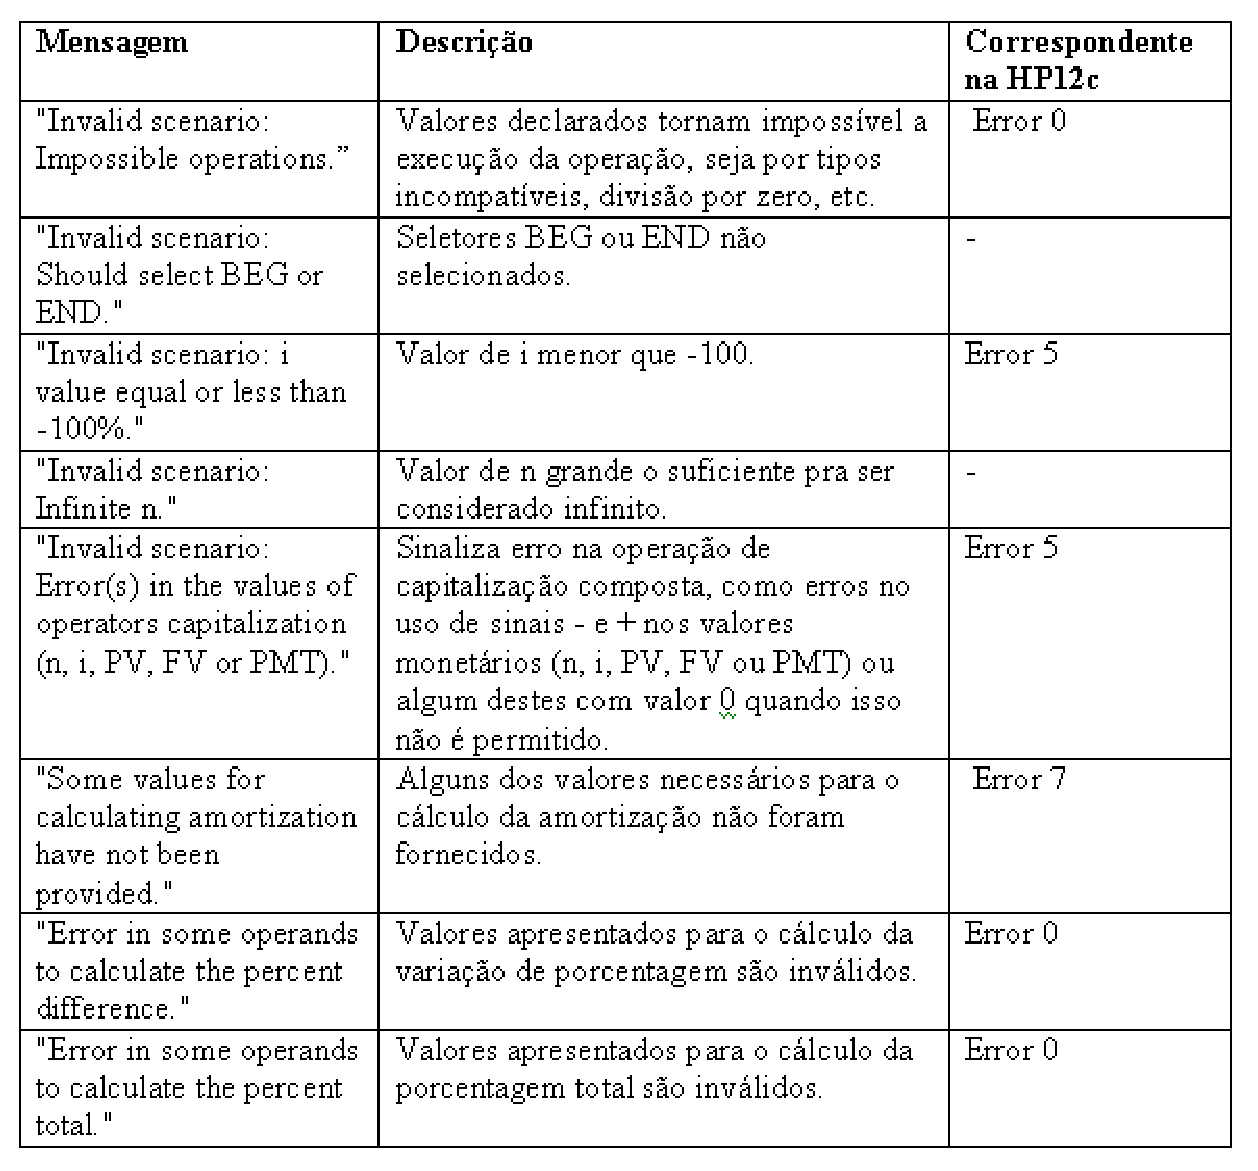
\includegraphics[scale = .7]{tabErro1.eps}
%  \includegraphics[scale=0.5]{bigchart.eps}
\caption{\it Mapeamento de Erros da Biblioteca}
\label{tabErros1} 
\end{figure}

\begin{figure}[!h]
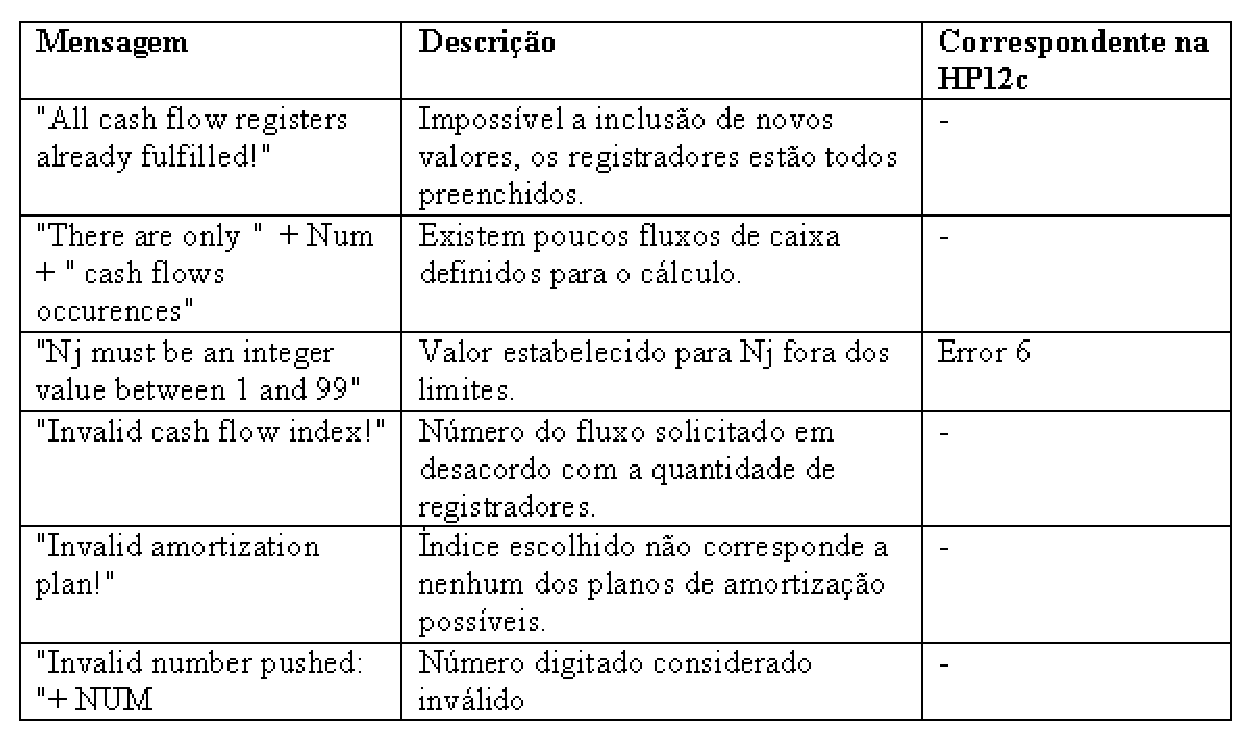
\includegraphics[scale = .7]{tabErro2.eps}
\caption{\it Mapeamento de Erros da Calculadora}
\label{tabErros2}
\end{figure}

\chapter{Diagrama de Classes} \label{DiagramaClasses}

Aqui temos a visualização dos principais componentes da calculadora financeira apresentados em um diagrama de classes. Os principais módulos e pacotes estão apresentados nas Figuras \ref{view} e \ref{model}.

\begin{figure}[!h]
\centering
 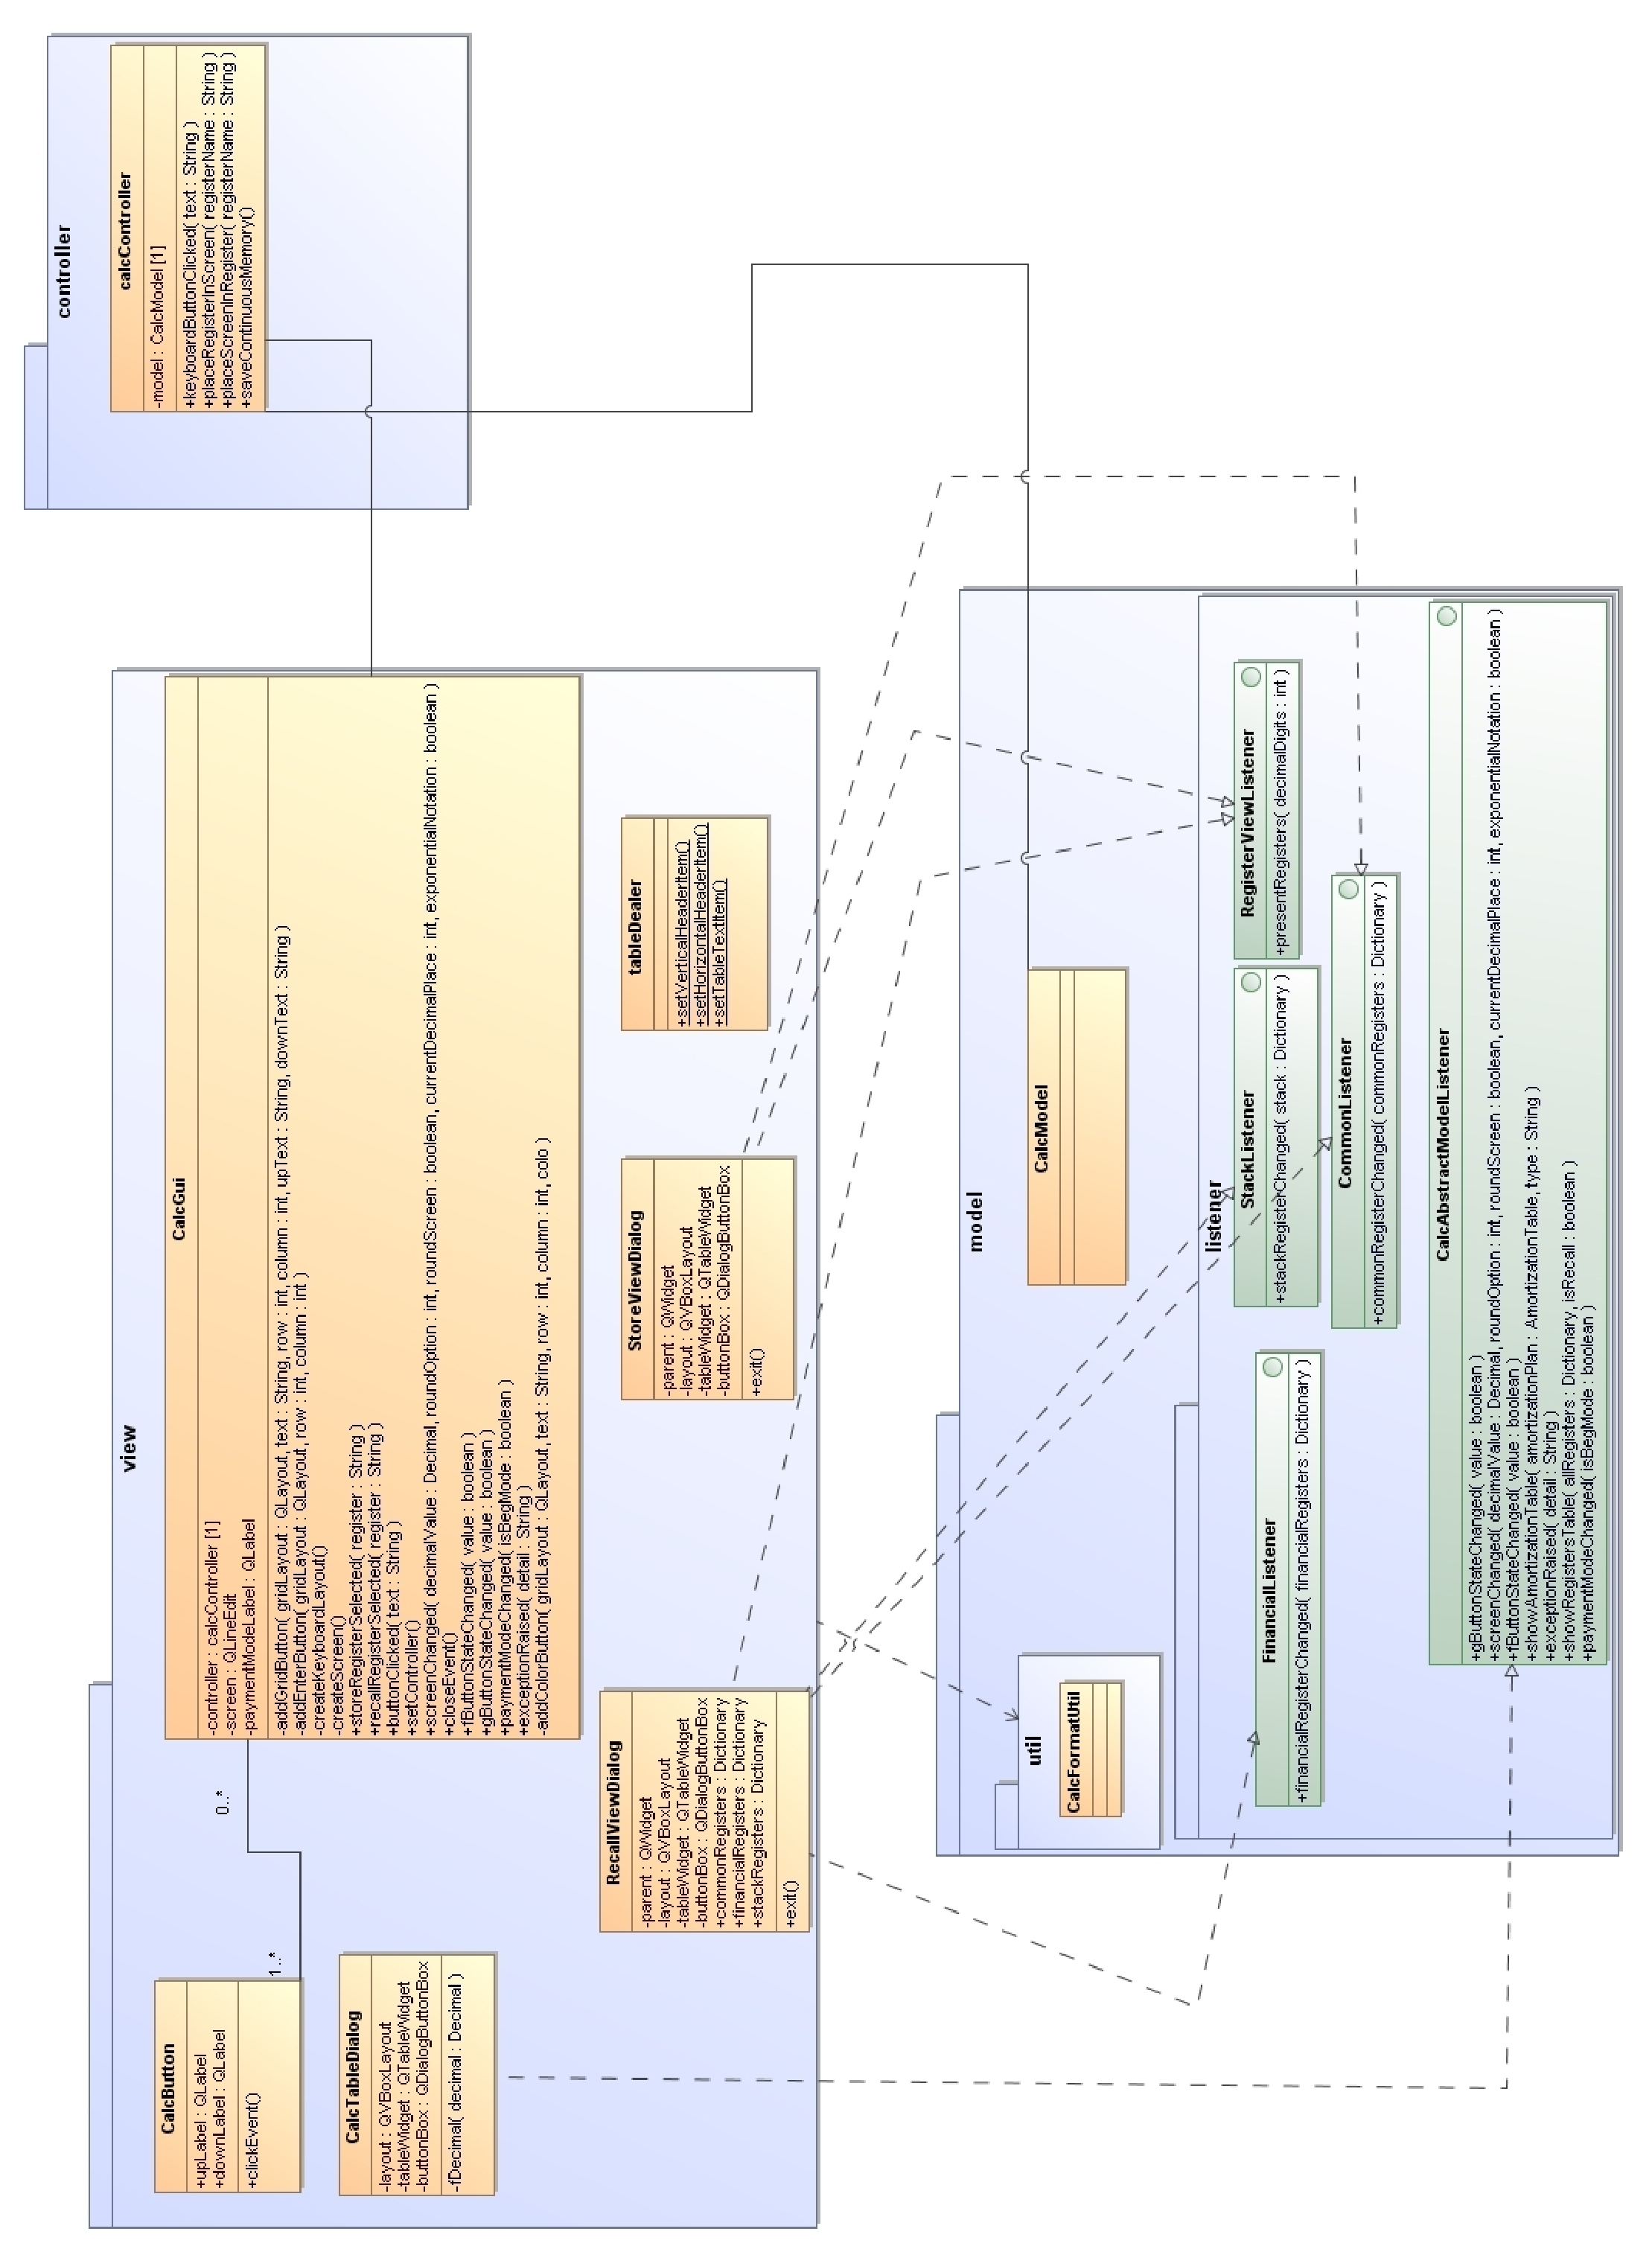
\includegraphics[scale=0.4]{Diagrama1.eps}
 \caption{\it Pacote view e controller e ligações com o pacote model.} \label{view}
\end{figure}

\begin{figure}[!h]
\centering 
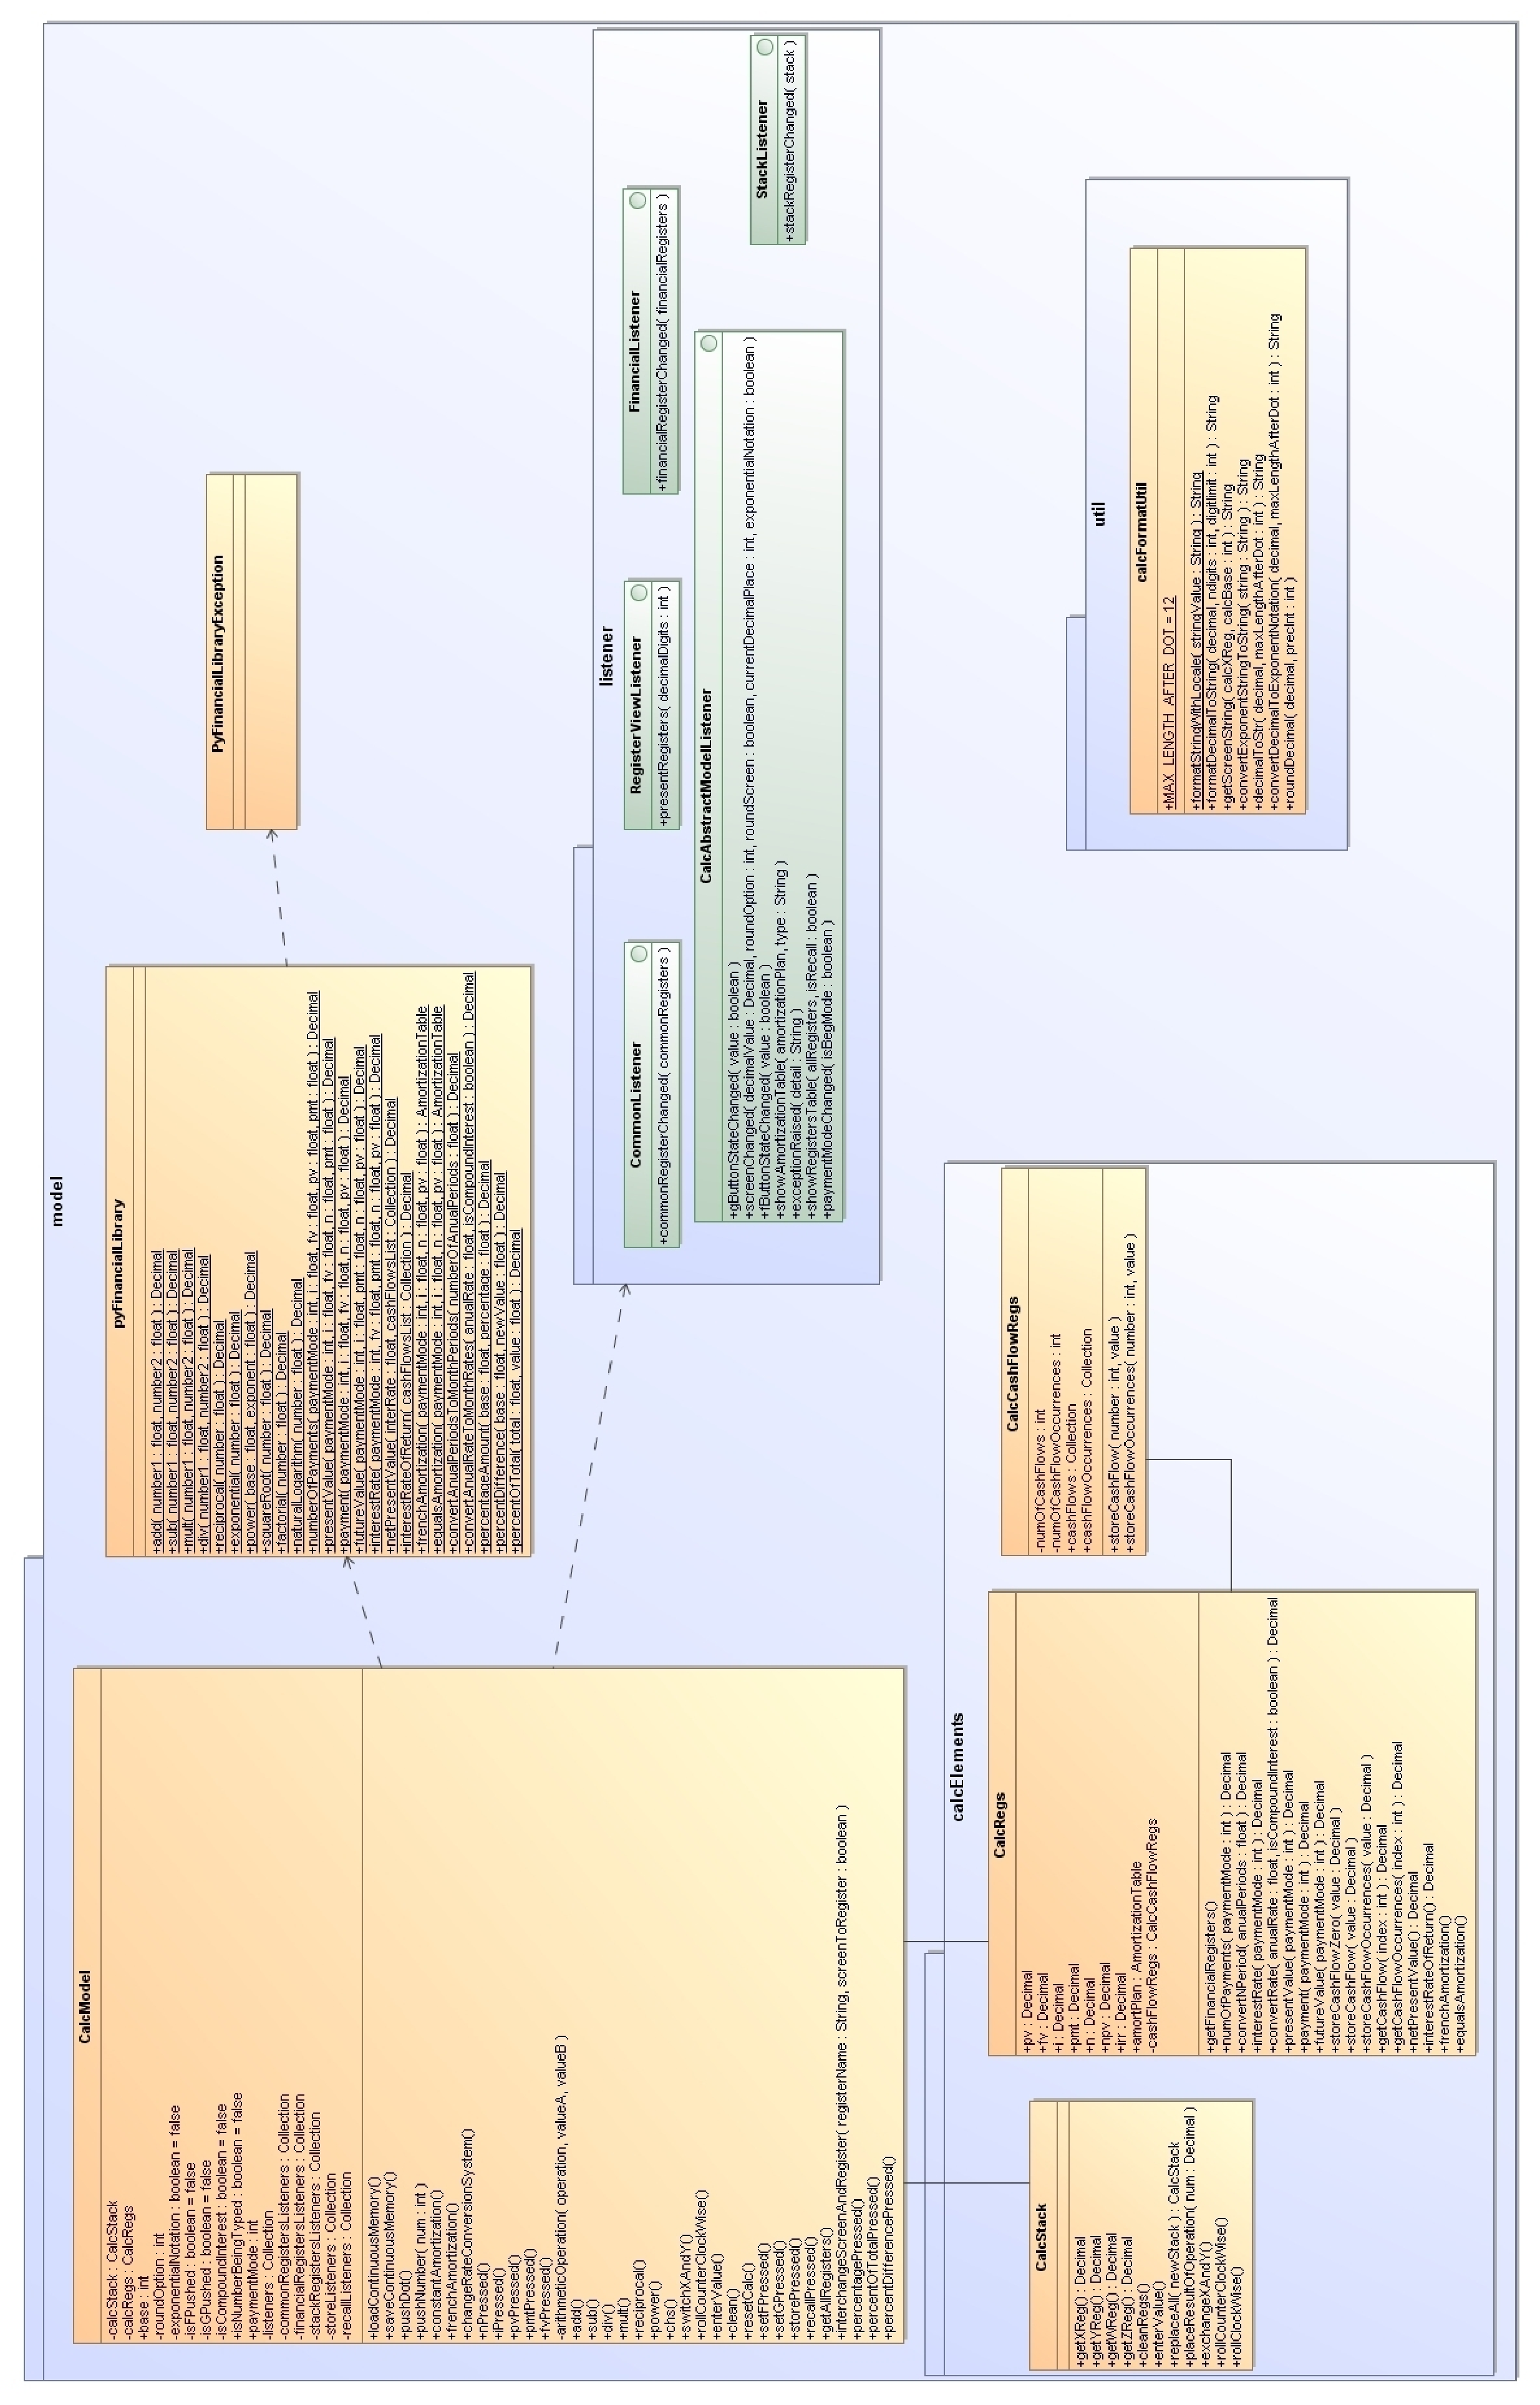
\includegraphics[scale=0.38]{model.eps}
 \caption{\it Pacote model.} \label{model}
\end{figure}

 \chapter{Telas da Aplicação}

\subsection{Tela Principal}

\begin{figure}[!h]
 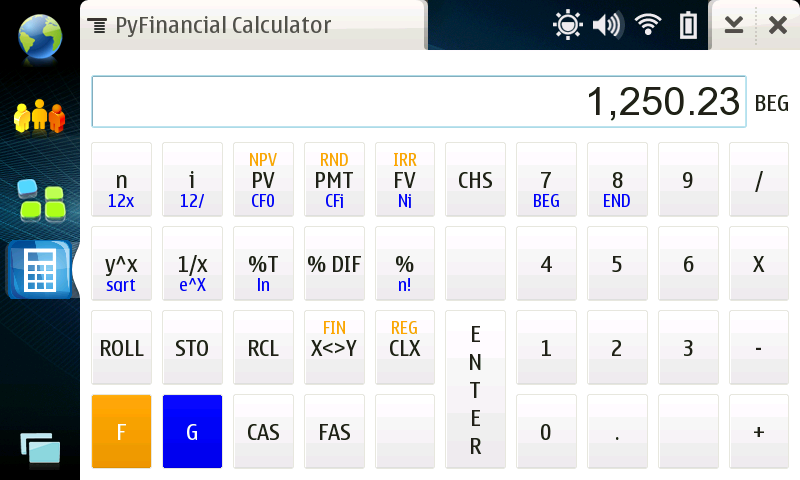
\includegraphics[height = 14cm]{tela_principal.png}
 \caption{\it Tela principal da calculadora.} \label{tab:tela_principal}
\end{figure}

Tela principal da aplicação que permite o usuário ter acesso a todas as funcionalidade
implementadas pela calculadora. É atraves do mostrador da calculadora que o usuário irá
receber o resultado da maioria das funcões.


\subsection{Tela de Exceção}

\begin{figure}[!h]
 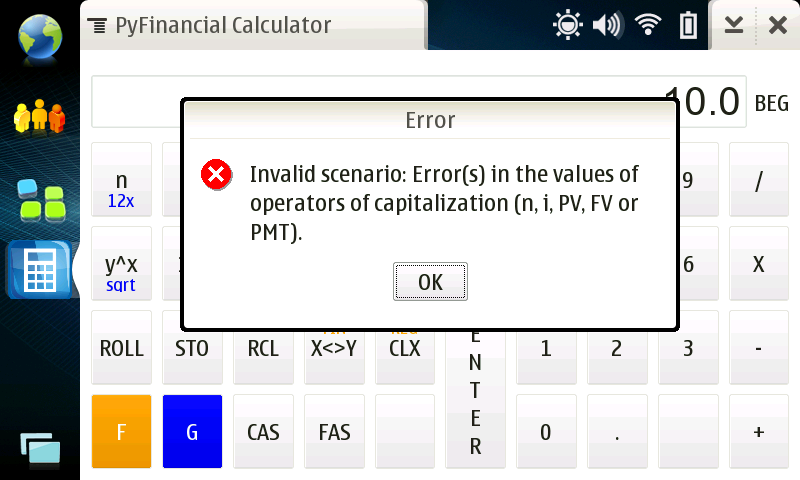
\includegraphics[height = 14cm]{tela_error.png}
 \caption{\it Tela de exceção.} \label{tab:tela_error}
\end{figure}

Tela principal após uma exceção ser gerada. Um box é aberto para mostrar ao usuário a
mensagem de erro.


\subsection{Telas de Amortização}

\begin{figure}[!h]
 \includegraphics[height = 14cm]{teal_cas.png}
 \caption{\it Tela de amortização constate.} \label{tab:tela_cas}
\end{figure}

\begin{figure}[!h]
 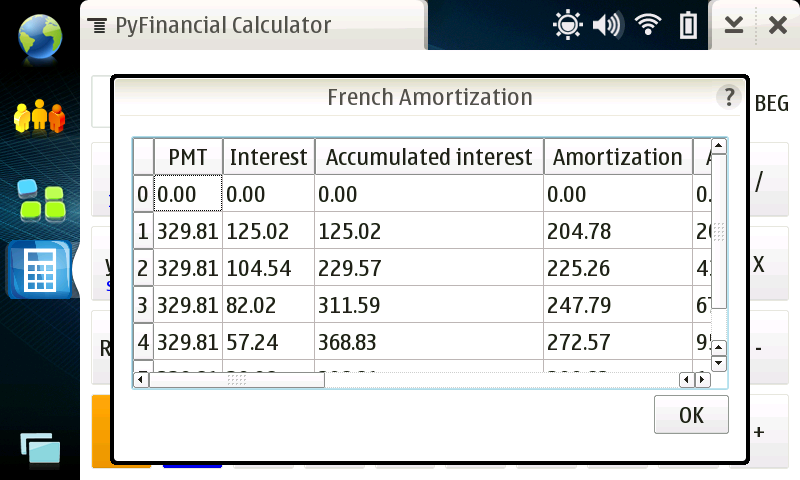
\includegraphics[height = 14cm]{tela_fas.png}
 \caption{\it Tela de amortização francesa.} \label{tab:tela_fas}
\end{figure}


As telas de amortização apresentam no formato de tabela o resultado de uma calculo de
amortização constate ou francesa.


\subsection{Telas de Recall}

\begin{figure}[!h]
 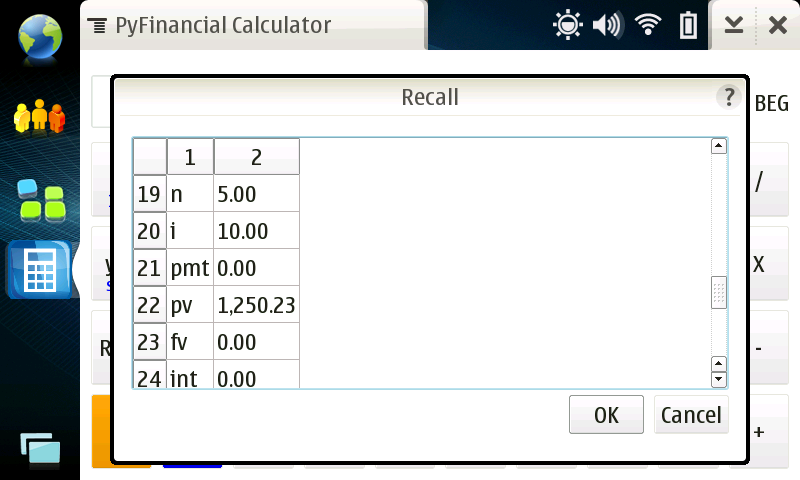
\includegraphics[height = 14cm]{tela_recall.png}
 \caption{\it Tela de recall de registradores.} \label{tab:tela_recall}
\end{figure}

A tela de Recall serve para o usuário selecionar um registrador da calculadora e o valor
dele será mandado para o mostrador quando o ele clicar em OK. Dessa forma, a pessoa poderá
utilizar o valor de um registrador em novos cálculos.

Existe também uma tela de Store, com o mesmo design da tela de Recall, que permite que o
usuário faça o inverso: armazene o valor do mostrador em um registrador.


% ------------------  Bibliografia  ------------------- %
%% Bibliografia

\bibliographystyle{sbc} % estilo de bibliografia
\bibliography{referencias.bib} % arquivos com as entradas bib.





\end{document}
